\documentclass[twoside, 12pt]{report}

\usepackage[
  a4paper,
  inner = 35mm,
  outer = 25mm,
  top = 25mm,
  bottom = 25mm,
  headheight = 16pt
]{geometry}
\linespread{1.5}

\usepackage{fancyhdr}
\pagestyle{fancy}
\fancyhf{}
\renewcommand{\headrulewidth}{0.5pt}
\renewcommand{\footrulewidth}{0pt}
\renewcommand{\chaptermark}[1]{\markboth{\thechapter.\ \MakeUppercase{#1}}{}}
\fancyhead[LE]{\leftmark}
\fancyhead[RO]{\leftmark}
\fancyfoot[C]{\thepage}

\usepackage[utf8]{inputenc}
\usepackage[magyar]{babel}
\usepackage{t1enc}

\pagenumbering{gobble}

\usepackage{graphicx}
\graphicspath{ {images/} }
\newcommand{\graphicswidth}{0.9\textwidth}

\renewcommand{\thefigure}{\arabic{figure}}
\renewcommand{\thetable}{\arabic{table}}
\usepackage{chngcntr}
\counterwithout{figure}{chapter}
\counterwithout{table}{chapter}

\usepackage[bottom]{footmisc}
\interfootnotelinepenalty=10000
\raggedbottom
\sloppy
\clubpenalty=3000
\widowpenalty=3000

\usepackage[
  backend=biber,
  style=alphabetic,
  sorting=nyt
]{biblatex}
\addbibresource{thesis.bib}

\usepackage[hidelinks]{hyperref}

\usepackage{amsfonts, amsmath, amssymb, amsthm}
\usepackage{blindtext} % TODO: Remove.
\usepackage{emptypage}
\usepackage{enumitem}
\usepackage{float}
\usepackage{makecell}
\usepackage[stretch=10]{microtype}
\usepackage{multirow}

\begin{document}

\begin{titlepage}
  \linespread{1.25}
  \begin{center}
    \begin{tabular}{ c c }
      \multirow{4}{*}{
        \hspace{-1.0cm}
        
\includegraphics[width=0.25\textwidth]{elte.png}} &
      {\sc \large \makecell{Eötvös Loránd Tudományegyetem}} \vspace{0.1cm}\\ &
      {\sc \large \makecell{Informatikai Kar}} \vspace{0.7cm}\\ &
      {\sc \makecell{Programozáselmélet és \\ Szoftvertechnológiai Tanszék}}
    \end{tabular}
    \vspace{4.0cm}
    \vspace{1.0cm}
    {\bf \Large Programkód-generálás természetes nyelvből \\
                mély neuronhálók használatával}
    \vspace{4.0cm}
    \vspace{1.0cm}
    \begin{tabular}{ l c l }
      {\it \large Témavezető:} &
      \hspace{4.0cm} &
      {\it \large Szerző:}\\
      {\large Várkonyi Teréz Anna} &
      \hspace{4.0cm} &
      {\large Dina Tamás Pál}\\
      egyetemi adjunktus, PhD &
      \hspace{4.0cm} &
      programtervező informatikus BSc\\
    \end{tabular}
    \vfill
    {\it Budapest, 2020}
  \end{center}
\end{titlepage}

\begin{center}
  \textbf{Szakdolgozat témabejelentő}
\end{center}

\thispagestyle{empty}

A szoftvertechnológia egyik központi célja a fejlesztési folyamatok gyorsítása és hatékonyabbá tétele. A komplex rendszerek gyakran egyszerűbb részekre bonthatók, amelyek könnyen és röviden megfogalmazhatóak természetes nyelv használatával is. Vizsgálatom célja olyan mesterséges intelligencia fejlesztése, amely így megadott feladatokat megoldó programrészleteket generál. A kutatás tárgyát azok a problémák alkotják, amelyek programozási tételek egyszerű alkalmazásával megoldhatók. Ez a strukturális megkötés lehetővé teszi a leggyakrabban előforduló problématípusok egységes megközelítését az általános felhasználhatóság jelentős sérülése nélkül.

A bemenő adatok nyelve az angol, a kimenő programrészletek nyelve a Python. A modelleket egy erre a célra elkészített BNF alapján generált adathalmazon tanított TranX neurális háló állítja elő. A szöveget először fel kell dolgozni, hogy minél jobban illeszkedjen erre a formális nyelvre. Az eredményesség vizsgálata kézzel összeállított példákon történik, a BLEU pontozási rendszer szerint.

A fejlesztési folyamat két jól elkülönülő részre bontható. Egyrészt szükséges a BNF nyelvtan definiálása, illetve az annak megfelelő mondatokat és a hozzájuk tartozó kódrészleteket legyártó generátor megírása. A komplex szövegek kezeléséhez olyan segédeszközöket kell felhasználni, mint például a SpaCy előtanított neuronháló, amelyet fejlett természetes nyelvi feldolgozásra terveztek. Másrészt a TranX további funckiók hozzáadására és konfigurációra szorul. A teljes folyamat megvalósításához szkripteket kell írni és köztes adatszerkezeteket kell meghatározni. A rendszer elemzése egyrészt teszteléssel, másrészt egy web API használatával történik, melyeket szintén implementálni kell.

A formális nyelvekhez, példageneráláshoz és a preprocesszáláshoz kapcsolódó teendőket Rikk Richárd látja el és ismerteti szakdolgozatában, míg a neurális hálókkal, azok kiértékelésével és az implementációval én foglalkozom, és ezek lesznek a dolgozatom fő témái.

\tableofcontents

\newpage
\pagenumbering{arabic}

\chapter{Bevezetés}

Az elmúlt évek során számos eredmény került publikálásra programozási feladatok automatikus megoldásával kapcsolatban. A megnövekedett érdeklődés mögött többek között a friss mesterséges intelligencia technikák sikerei, a szabadon elérhető kódbázisok gyarapodása és a rendelkezésre álló számítási kapacitás ugrásszerű növekedése állnak. Ezek a tendenciák teszik lehetővé, hogy sorra dőljenek meg az elterjedt viszonyítási teszteken elért rekordok, és hogy egyre közelebb kerüljön az éles környezetben történő sikeres felhasználás lehetősége is.

Az automatikus programozásra képes szoftverek jelentős gyakorlati haszonnal kecsegtetnek. A programozók munkájának intelligens megoldásokkal történő támogatása jelenleg is figyelemre méltó potenciállal rendelkezik mind a produktivitás, mind a programhelyesség növelése terén. A Microsoft által fejlesztett IntelliCode \parencite{Mic18a} például több ezer szabad forráskódú projekt alapján képes az adott kontextusnak megfelelő javaslatokat tenni a kód folytatására, a DeepCode \parencite{Dee16a} elnevezésű szoftver pedig segíthet gyakran előforduló szemantikai hibák kiküszöbölésében. Ezeket az eszközöket már most is fejlesztők ezrei használják, és a predikciók pontosságának javulásával az elterjedtségük is nőni fog.

Mindezek ellenére az IntelliCode és a DeepCode, ugyan nagyon hasznosak, nem képesek önálló programalkotásra. A programszöveg elemzésével mintákat ismernek fel, de nincs kapcsolatuk a programozó által megoldandó feladathoz. Ezzel szemben az automatikus programszintézis kevésbé a már megírt programra, sokkal inkább egy feladatleírásra épít, az alapján generálva a programszöveget, amellyel a feladat megoldására törekszik. A szintetizálás folyamata szorosan fűződik az emberek által kialakított fogalmak és összefüggések megértéséhez, mely képességgel a jelenleg elérhető fejlesztéstámogató rendszerek nem rendelkeznek.

Összehasonlítva a programszöveg-elemzéssel, a legnagyobb nehézséget az okozza a programszöveg-generálás problémájának megoldásában, hogy a feladatok leírásai nagyon ritkán érhetők el olyan formában, amelyet precízen lehet értelmezni számítógépek segítségével. Az emberek által leggyakrabban használt feladatspecifikációs-eszközök a természetes nyelvek, melyekről köztudott, hogy a számítógépes feldolgozásuk (natural language processing) kifejezetten nehéz \parencite{Pra10a}.

Természetesen léteznek formális eszközökkel definiált feladatok megoldására irányuló törekések is \parencite{GCM20a}. Ekkor az input jól körülhatárolható szintaxissal és szemantikával rendelkezik, a problématér elemeiről pedig a keretrendszer biztosít a priori ismereteket. Ennek a megközelítésnek az előnye, hogy az elvárt viselkedés nagyobb precizitással írható le, és hogy a "feladat", "megoldás" valamint "program" fogalmak akár matematikai eszközökkel is megadhatók.

Dolgozatom a természetes nyelven alapuló programszintézis kérdésével foglalkozik. Egy keretrendszer kerül bemutatásra, amely alkalmas programok különböző reprezentációk közötti átalakítására, ezáltal lehetővé téve akkurátusabb generáló algoritmusok fejlesztését. Az automatikus programozás egyik nagy kihívása az, hogy a végeredmény meg kell feleljen a programozási nyelv szigorú lexikális és szintaktikai szabályrendszerének. Ezek a szabályok olyan megkötést jelentenek, amelyet minden esetben hibátlanul teljesíteni kell, de a probléma legérdekesebb eleméhez, a szemantikai helyességhez nem visz közelebb. Különösen igaz ez a probabilisztikus modellekre, amelyek gyakran nehezen alkalmazkodnak az ilyen szabályok betartásából eredő megnövekedett komplexitáshoz.

Szerencsére léteznek módszerek ennek a problémának a kiküszöbölésére. A programozási nyelvek lexikális és szintaktikai rendszerei jól leírhatók a formális grammatikák eszközeivel, ezáltal automatikusan és determinisztikusan kezelhetők. Ez kihasználható, ha a programgenerálás során nem a programszöveg, hanem annak egy szemantikailag ekvivalens de szintaxistámogatott reprezentációja kerül előállításra. A szintaxistámogatottság itt azt jelenti, hogy a reprezentáció gondoskodik a szintaxishelyesség biztosításáról a generáló algoritmus helyett.

Alkalmas köztes reprezentációt jelentenek a szintaxisfák. A szintaxisfák explicit módon tartalmazzák a nyelv grammatikájának nemterminálisait, így a programszintézis sokkal strukturáltabb módon folyhat le: a generáló algoritmusnak nem arról kell döntenie, hogy egy adott ponton zárójel következzen-e, hanem arról, hogy paraméterlista, zárójeles kifejezés, vagy esetleg valami más. A végeredmény tekintetében mindkét eset ekvivalens, de az utóbbi jelentősen hasznosabb heurisztikák alkalmazását teszi lehetővé, miközben kizárólag jól formulált programok előállítását engedi.

A legjobb eredményeket jelenleg a felügyelt tanítással felkészített neurális hálók produkálják \parencite{KD19a}, nem kis mértékben annak köszönhetően, hogy ez a technika a közelmúlt legígéretesebb eszköze a természetes nyelvfeldolgozás területén. Szintaxistámogatott reprezentációk alkalmazásával némely fejlett modell képes kifejezetten komplex összefüggések felismerésére is a szöveges feladatleírások és az azokat megoldó programok között. Ezen megközelítés segítségével \textcite{RSK17a} közel négyszer több tökéletes találatot ért el a bonyolult példákat tartalmazó Hearthstone adathalmazon \parencite{Dee16b}, mint a korábbi legjobb modellnek számító \textcite{Lin+16a}.

Az egyik legsikeresebb szabad forráskódú state-of-the-art implementáció a TranX \parencite{YN18a}. Ez egy úgynevezett tranzíciós rendszert (transition system) használ, innen ered a neve is: TRANsition-based abstract syntaX parser (átmenet-alapú absztrakt szintaxis elemző). A TranX a \textcite{RSK17a} által megalkotott abstract syntax network (ASN) hálóarchitektúrának egy továbbgondolása, közös alapelvük, hogy az adott programozási nyelvnek megfelelő összes szintaxisfa közül az egyiket procedurálisan építik fel, minden szintaxisfa-építő lépésnél egy neurális hálót, mint heurisztikát alkalmazva választva ki, hogy melyik folytatás lehet a leghelyesebb.

A dolgozatom fő kontribúciója egy új nyelvtankezelési módszertan bevezetése. A TranX által alkalmazott tranzíciós rendszer ugyan nyelvfüggetlen, mivel a szintaxisfákat a programozási nyelv konkrét szabályaitól függetlenül tárolja és kezeli, de a programszöveg és szintaxisfa közötti oda-vissza fordítás erősen nyelvfüggő feladatát nem képes automatikusan megvalósítani. Ez azt jelenti, hogy ha valaki a TranX-ot egy új programozási nyelvre szeretné felhasználni, akkor a tranzíciós rendszerhez további programrészeket kell írnia, amely rengeteg munkával járhat. Implementálnia kell úgynevezett parser és unparser programokat, amelyek képesek a programszöveget a TranX által specifikált formába feldolgozni és átalakítani, és ez a feladat egyáltalán nem számít triviálisnak.

Az általam bevezetett rendszer leveszi ezt a terhet a felhasználó válláról, és egy teljes mértékben általánosított megoldást nyújt. Lehetővé teszi a teljes átalakítási folyamat elvégzését az eredeti program kiegészítése nélkül, kizárólag egy, a programozási nyelv szabályait definiáló nyelvtanfájl megadásával. A programom hasonló feladatot old meg, mint a GNU lex-yacc programcsomag, de néhány problémára alternatív megoldásokat és módszereket vezet be. Tulajdonképpen egy fordítóprogram-generátorról van szó, csak a fordítás folyamata megáll a köztes reprezentációként használt szintaxisfánál, és nem állít elő assembly kódot.

A dolgozatom keretében nem csupán ezt a generátort, hanem illusztrációs céllal egy teljes programszintetizátort és egy példa adathalmazt is elkészítettem. A példák angol nyelvű feladatleírásokat és Python nyelven írt programokat tartalmaznak. A program először feldolgozza a Python nyelvet definiáló nyelvtanfájlt, majd ez alapján előállít egy teljes értékű fordítóprogram-frontendet, valamint egy olyan programot, amely képes a Python szintaxisfákat programszöveggé konvertálni. Ezután a feladat-megoldás párok betáplálhatók egy szekvencia-párosító encoder-decoder neurális hálóba, amely tanítás után felhasználható predikciók előállítására tetszőleges bemenet esetén.

A programom a SASN nevet kapta, amely egy mozaikszó, a Simple Abstract Syntax Network rövidítése. Megjegyzendő, hogy a jelen dolgozathoz mellékelt szoftver nem pontosan egy absztrakt szintaxis háló, hanem egy egyszerűsített modell. A keretrendszerrel bármilyen predikciós algoritmus használható, de a nyelvtani transzformációkból eredő előnyöket főleg az ASN-ek tudják kihasználni. További vizsgálat tárgyát képezheti, hogy a meglévő jól teljesítő ámbár rendkívül összetett rendszerek, mint amilyen a TranX is, hogyan viselkednek ebben a környezetben, ez azonban már túlmutat a dolgozat keretein.

A dolgozatomat az MLforSE (Machine Learning for Software Engineering) elnevezésű EFOP-támogatott kutatás keretében készítettem el. A témabejelentőt a kutatás egy korai fázisában írtam, így azóta sok minden megváltozott a választott megközelítések terén. Az eredeti terv szerint már létező megoldásokat alkalmaztam volna egy új adathalmazra, azaz kevesebb lett volna a hozzáadott érték és a saját fejlesztés, ezáltal a dolgozatom is inkább esettanulmány-jellegű lett volna. A kutatás során azonban felmerültek bennem a fent ismertetett komplexebb kérdéskörök, így jutottam el végül a nyelvtani generátor valamint egy saját predikciós modell implementációjáig. Emiatt némely konkrétum, amelyet eleinte belefoglaltam a témabejelentőmbe, nem került felhasználásra, így a SpaCy\footnotemark{} és TranX hálók, a BLEU pontozási rendszer \parencite{Pap+02a} és a web API nem képezik részét a dolgozatomnak.

\footnotetext{https://spacy.io/}

A példa adathalmaz feladat-megoldás párokat tartalmazó JSON fájljait Rikk Richárd hallgatótársam állította elő a saját szakdolgozata keretében. Felírt egy BNF \parencite{Bac59a} sablont, amely segítségével feladatleírások és azokat megoldó programok generálhatók. A BNF leírás különböző programozási tételek \parencite{Gre10a} köré épül fel, ezáltal a példák jól strukturáltak és garantáltan helyesek.

A további fejezetekben először felvezetem az automatikus programszintézis szemantikai elemzés nevű részterületét, majd bemutatom a probléma néhány lehetséges modellezési megközelítését. Ezután bemutatom azokat a jelentésreprezentációkat, amelyek a programszöveg és a probléma modell által jól megragadható adatszerkezetek közötti konverzió során jönnek létre. Az elméleti összefoglaló végső szakaszában a megalkotott modell megoldási lehetőségeiről számolok be. A dolgozat további részét a felhasználói dokumentáció, majd a fejlesztői dokumentáció, és végül egy összegző áttekintés képezik.

\chapter{Elméleti háttér}

A következő fejezetek formális bevezetést nyújtanak a dolgozatban feldolgozott főbb témákhoz. A felhasználói és a fejlesztői dokumentáció használata előtt ajánlott áttekinteni az itt leírtakat, de azok beható ismerete nem szigorú előfeltétele a szoftver használatának. A program fő célközönségét azok az informatikusok képezik, akik szeretnék a SASN nyelvtani keretrendszerét saját kutatásaik céljaira felhasználni, ebből kifolyólag számos alapfogalom magyarázat nélkül kerül említésre.

Az alábbiakban bemutatásra kerülő témakörök a számításelmélet, a formális nyelvek és fordítóprogramok, valamint a mesterséges neuronhálók területeinek metszetében helyezkednek el. Ezek a területek számos esetben hivatkoznak általános matematikai fogalmakra és összefüggésekre is. Az alábbi lista a teljesség igénye nélkül foglalja össze a dolgozat, az implementáció valamint minimális mértékben a hivatkozott szakirodalom megértéséhez szükséges előismereteket. Mivel mindezek bevezetése nagyon hosszadalmas lenne, ezenfelül elsajátításuk részét képezi a programtervező informatikus alapszak sillabuszának, így a dolgozatban nem kerülnek részletesebben kifejtésre.

\begin{itemize}[noitemsep]
  \item Halmazelméleti alapok, halmazok számossága. Relációk és függvények, valamint tulajdonságaik. Ekvivalenciaosztályok, részbenrendezések.
  \item Kombinatorika: Elemek variációja. Valószínűségszámítás: Feltételes valószínűség, láncszabály, teljes valószínűség tétele.
  \item Algoritmusok: Mohó algoritmus, "brute force", backtracking. Szélességi keresés, nyalábkeresés \parencite{Red77a}, preorder bejárás. Heurisztika, problématér.
  \item Gráfelmélet: Irányított gráf, fa, út, séta, kör. Csúcs kifoka, befoka. Aciklikus gráfok.
  \item Formális grammatikák: Véges nyelvtan, szó, részszó, mondatforma, szóprobléma, levezethetőségi reláció. Chomsky-hierarchia. Reguláris kifejezések. Aciklikus nyelvtanok. BNF \parencite{Bac59a}, EBNF \parencite{Wir77a}, ABNF \parencite{CO08a}. Epszilonmentesítés, bal-rekurzió.
  \item Fordítóprogramok: Lexikális nyelvtan, szintaxis, szemantika. Token, szintaxisfa. Operációk, precedencia. Parsing, unparsing. Rekurzív leszállás módszere. LL(1) elemzés, FIRST és FOLLOW halmazok. PEG nyelvtan \parencite{For04a}.
  \item Gépi tanulás: Tanulási technikák: felügyelt, induktív, mély. Mesterséges neuronháló. Hibafüggvény, softmax és ReLU kimeneti függvények. Rekurrens réteg. Encoder-decoder architektúra. LSTM \parencite{HS97a} és GRU \parencite{Cho+14a} cellák. Neurális figyelem (attention). Túlilleszkedés (overfitting).
\end{itemize}

\section{Problémafelvetés}

\subsection{Szemantikai elemzés}

A szemantikai szövegelemzés (semantic parsing) feladata természetes nyelvű lekérdezésekhez (natural language query, NLQ) formális jelentésreprezentációk (formal meaning representation, FMR) párosítását jelenti. Ennek formális megfogalmazása megadható a $\varphi \subseteq NLQ \times FMR$ reláció megtalálásaként, ahol egy adott $q \in NLQ$ lekérdezésre az $r \in FMR$ reprezentáció megfelel $q$-nak, ha $r \in \varphi(q)$.

Jelen dolgozat keretében a $q = w_{1} ... w_{|q|} \in NLQ$ lekérdezés egy adott természetes nyelv szabályai szerint helyesen formulált szöveg, szavak szekvenciájaként kifejezve. Egy $r = s_{1} ... s_{|r|} \in FMR$ reprezentáció egy adott formális nyelvhez tartozó terminális szimbólumok szekvenciája.

A $\varphi$ által megragadott viszony szemantikai jellegű. Amikor egy $(q, r)$ rendezett pár eleme a $\varphi$ relációnak, az azt jelenti, hogy $q$ emberek által megragadott jelentéstartalma megfeleltethető $r$ számítógépek által feldolgozható jelentéstartalmával.

\subsection{Intenció elemzés}

Az intenció elemzés (intent parsing) a szemantikai szövegelemzés egy speciális esete. Intenció elemzés során $q$ jelentéstartalma az intenció tárgya, azaz a tevékenység vagy effektus amely végbemenetelére az intenció irányul. A szemantikai elemzés keretében előállított reprezentáció olyan kell, hogy legyen, hogy az eredeti tevékenység vagy effektus reprodukálható (és végrehajtható) legyen kizárólag a reprezentáció alapján.

Az intenció elemzés alkalmazható a programok írásakor végbemenő szemantikai tranzíció modellezésére. A programozó rendelkezik egy céllal, amelyet a programon keresztül a számítógéppel végrehajtatni kíván. Ennek a célnak egy természetes nyelven való megfogalmazása megtörténik a program implementációja előtt, de ez a meghatározás csak nagyon nehezen formalizálható.

\subsection{A szemantikai reláció vizsgálata}

Érdemes $\varphi$ néhány alapvető tulajdonságát megjegyezni:

\begin{itemize}[noitemsep]
    \item $\varphi$ nem bal-totális: Nem minden lehetséges lekérdezés számít helyes feladatleírásnak, és nem minden lekérdezhető feladatnak van megoldása.
    \item $\varphi$ jobb-totális: Minden helyes programhoz tartozik legalább egy megfelelő feladatleírás.
    \item $\varphi$ nem bal-egyértelmű: Egy program több, mint egy feladatleírással is rendelkezhet.
    \item $\varphi$ nem jobb-egyértelmű: Egy természetes nyelvű lekérdezéshez több azt megoldó program is tartozhat.
\end{itemize}

\section{A probléma modellezése}

\subsection{Naív formuláció}

A feladat eredeti megfogalmazása intuitívan elvezet a legegyszerűbb probléma modellhez, amely a kimeneti szekvenciák szintjén dolgozik, ezáltal nem igényel introspekciót a formális nyelv szabályaiba. A problémát ilyen megközelítéssel megoldó algoritmusok az összes $NLQ$ és $FMR$ közötti reláció halmazán ($NLQ \times FMR$) végeznek keresést egy adott $q$ lekérdezésre. Az algoritmusok visszatérési értéke egy olyan pár, amelynek első komponense $q$.

Az egyetlen feltétel, amely a naív formuláció melletti terminációhoz szükséges, az az, hogy $NLQ \times FMR$ számossága véges legyen. Ez teljesíthető, ha a megoldások keresése csupán $NLQ \times FMR$ egy véges részhalmazán történik, vállalva, hogy ekkor az algoritmus fals negatív eredményeket produkálhat. (Ez a feltétel lazítható megszámlálhatóan végtelen számosságra is, ha $\varphi$ bal-totális, azaz ha garantált, hogy $\forall q \in NLQ: \exists r \in FMR: (q, r) \in NLQ \times FMR$. Ekkor ugyanis minden megoldás véges lépésben elérhető, csupán nem helyezhető felső határ a szükséges keresési lépések számára.)

Ennek a formulációnak az előnye, hogy rendkívül egyszerű, valamint, hogy mivel minden vizsgált $r$ reprezentáció eleme $FMR$-nek, így csak olyan eredmények kerülhetnek kiválasztásra, amelyek garantáltan szintaktikailag és szemantikailag helyesek. Hátránya, hogy a teljes $NLQ \times FMR$ reláció előzetes ismerete szükséges hozzá, ami az általános esetben gyakorlatilag lehetetlen.

A naív formuláció nem feltétlenül jelent egyszerű algoritmust. A bemenet tetszőlegesen bonyolult módon elemezhető, a megkötések a felismert karakterisztikák felhasználásában jelentkeznek. Ilyen szempontból ez a technika inkább egy klasszifikációs vagy információszerzés (information retrieval) feladatot old meg. Példaként megemlíthető lenne egy olyan program, amely egy adott természetes nyelvű feladatleírásra megállapítja, hogy melyik programozási tétel oldaná meg azt.\footnotemark{}

\footnotetext{Ez a feladat nem azonos az MLforSE projekt keretében vizsgált feladattal. Ez esetben a rendszer explicit tudással rendelkezik a programozási tételek struktúrájáról, és a bemenet jellemzői alapján választja ki azok paramétereit (például a felsorolt gyűjteményt, az összegfüggvényt, stb.).}

\subsection{Tokenvariáció-alapú formuláció}

A szemantikai elemzés egyik klasszikus megközelítési formája a kimenetek terminális szimbólumok szintjén történő előállítása. Mivel $FMR$ általában jelentősen nagyobb számosságú, mint az alapját képező terminális ábécé, így az utóbbi kezelése egyszerűbb lehet. A legfontosabb különbség a naív megoldáshoz képest az, hogy a keresés és vizsgálat egysége nem egy teljes szekvencia, hanem a szekvencia egy eleme, tehát nőtt a granularitás, ezáltal több tulajdonság (feature) biztosított az ilyen elven működő megoldó algoritmusok számára, például heurisztikákban történő felhasználás céljára.

A kimenetek előállítása egyszerű variációval történik. Az összes lehetséges szó (az ábécé elemei) közül kell kiválasztani néhány terminálist a megkívánt sorrendben. A terminális ábécé elemei programozási nyelvek esetén tokenek, ezért a modell nevezhető tokenvariáció-alapú formulációnak. A módszer visszavezeti a teljes szekvencia előállításának problémáját a szekvencia elemeinek sorrendben történő előállításának kompozíciójára.

Ilyen megközelítés mellett az általánosabb feltétel ($|NLQ \times FMR| < \infty$) két részfeltételre szűkíthető: legyen az ábécé számossága véges, valamint az előállított sorozatok hossza rendelkezzen véges felső határral.

Ez a formuláció továbbra is egyszerű, azonban nem feltétlenül eredményez mindig szintaktikailag helyes reprezentációkat (nem minden tokensorozat helyes). Erre megoldást jelenthet, ha létezik gyors algoritmus a szóprobléma eldöntésére. Értelemszerűen a hibásan formulált válaszok elfogadása is egy lehetséges megközelítés. Ez a technika különösen elterjedt a természetes nyelvek közötti fordítás esetében \parencite{BCB15a}, mivel a lehetséges input-output párok száma túl nagy, valamint a természetes nyelvek szintaxisa bonyolultabb (és vitatottabb), mint a programozási nyelveké.

\subsection{Gráfalapú formuláció}

Legyen $(N, \Sigma, P, S)$ egy véges grammatika, úgy, hogy $FMR = \{ r \in \Sigma^{*} \ | \ S \Rightarrow^{*} r \}$. Tekintsük a $G = (V, E)$ irányított gráfot, ahol a csúcsok a $V = \{ \alpha \in (\Sigma \cup N)^{*} \ | \ S \Rightarrow^{*} \alpha \}$ mondatformáknak, az élek az $E = \{ (\alpha_{1}, \alpha_{2}) \in V \times V \ | \ \alpha_{1} \Rightarrow \alpha_{2}  \}$ levezethetőségi relációnak felelnek meg. A $q$-hoz $r \in FMR \subseteq V$ reprezentációt párosító leképezés kiszámítása ekvivalens egy $S \in V$-ből induló, megfelelő $r \in \varphi(q) \subseteq V$-be tartó út megtalásával.

Ez a formuláció egy gráf modellt ad a problémának, amelyre egyaránt alkalmazhatók klasszikus heurisztikák és mesterséges intelligencia technikák. Előnye, hogy a gráf csupán szintaktikailag helyes programok előállítását engedi, valamint, hogy a formális jelentésreprezentációt a nyelvtani alkotóelemei szintjén kezeli (azaz például nemterminális szimbólumokkal is foglalkozik), ezáltal fontos grammatikai összefüggésekre is építhet heurisztikát. Fő hátránya a komplexitása, valamint az, hogy az $FMR$ grammatikája ismert kell legyen, így például természetes nyelvek esetén nem alkalmazható.

Három oka lehet annak, hogy egy útkeresési algoritmus nem terminál: nevezzük ezeket a "végtelen szélesség", a "végtelen mélység", valamint a "végtelen ciklusok" problémájának.

\textbf{\textsc{Végtelen szélesség}}\ \ \ A "végtelen szélesség" problémája pontosan akkor merül fel, ha $\exists v \in V: |deg^{+}(v)| \geq |\mathbb{N}_{0}| $. A gráf modell alapját képező nyelvtan segítségével ez felírható úgy, hogy $\exists \alpha \in V : |\{ \beta \in V \ | \ \alpha \Rightarrow \beta \}| \geq |\mathbb{N}_{0}|$. Nem triviális megadni, hogy pontosan mikor teljesül ez a feltétel, azonban a probléma elkerüléséhez elegendő azt biztosítani, hogy $ \forall \alpha \in V : |\alpha| < |\mathbb{N}_{0}|$. Az elégséges feltétel bizonyítása onnan következik, hogy ebben az esetben csak véges számú részszó van $\alpha$-ban, amelyből véges számú levezetési szabály alapján csupán véges számú új szót lehet alkotni.

\textbf{\textsc{Végtelen mélység}}\ \ \ A "végtelen mélység" problémája pontosan akkor merül fel, ha létezik végtelen hosszú út a gráfban, azaz ha $\exists \alpha, \beta, \gamma \in V, \beta \neq \varepsilon \, \lor \, \gamma \neq \varepsilon: \alpha \Rightarrow^{+} \beta \alpha \gamma$. Ehhez végtelen számú csúcs megléte szükséges, ezáltal $|V| < |\mathbb{N}_{0}|$ biztosításával a probléma kiküszöbölhető. Érdemes megjegyezni, hogy véges nyelvtanban $(\exists n \in \mathbb{N}_{0} : \forall \alpha \in V : |\alpha| < n) \Rightarrow (|V| < |\mathbb{N}_{0}|)$.

\textbf{\textsc{Végtelen ciklusok}}\ \ \ Nyelvtani deriváció során pontosan akkor kerülhet az algoritmus végtelen ciklusba, ha a gráf tartalmaz kört, azaz létezik $(e_{1}, e_{2}, ..., e_{n}) \in E^{n}$ nem üres séta $(v_{1}, v_{2}, ..., v_{n}, v_{1}) \in V^{n+1}$ csúcs szekvenciával. Legyen $\alpha$ a $v_{1}$-nek megfelelő mondatforma. Ekkor az előbbi feltétel ekvivalens azzal, hogy $\alpha \Rightarrow^{+} \alpha$ a formális grammatikában. Triviális, hogy ha $G$ egy fa, akkor nem tartalmazhat kört. Általánosabb feltételek meghatározása az aciklikus nyelvtanok tárgykörébe tartozik, amelynek néhány főbb eredménye: (1) a reguláris nyelvtanok mindig aciklikusak\footnotemark{} \ (2) a környezetfüggetlen nyelvtanok mindig veszteségmentesen átalakíthatók aciklikus nyelvtanokká \parencite{Aar92a} (3) az aciklikus környezetfüggetlen nyelvtanok általánosíthatók aciklikus környezetfüggő nyelvtanokká \parencite{Aar92a} (4) az aciklikus környezetfüggő nyelvtanok családja megegyezik a szigorúan monoton környezetfüggő nyelvtanok családjával \parencite{NW01a}. Bármely nyelvtan, amely ezen kategóriák egyikébe esik, nem tartalmaz kört. Mivel minden véges nyelv reguláris, ha $|V|$ véges, akkor $G$ körmentes.

\footnotetext{Mivel egy reguláris nyelvtan szigorúan monoton is, így ez következik (4)-ből.}

\section{Jelentésreprezentációk}

A három bemutatott probléma modell közül az absztrakt szintaxis hálók az utóbbit, azaz a teljes szintaxis ismeretére alapozó útkeresési formulációt alkalmazzák. A jelen dolgozat keretében elkészített modell is az ott bevezetett fogalmakra épít, de a neurális hálónak más szerepet ad. A problémát megoldó algoritmusok részletezése előtt azonban fontos kitérni a felmerülő reprezentációs formákra, valamint a köztük fennálló átmenetekre, mivel ezek teszik lehetővé a szintaxistámogatott generálást.

Annak ellenére, hogy az elvárt végkimenet Python kód, érdemesebb köztes adatszerkezeteket alkalmazni. Ennek az az oka, hogy a gráf modell csúcsai mondatformák, és nem csupán szavak, így nem mindegyik csúcshoz jut annak megfelelő programszöveg. A generálás során mégis szükséges ezeket a levezetés közben előforduló ideiglenes elemeket kezelni, és ez veti fel az igényt az alábbi diszkusszióra.

\subsection{Szöveges kódrészletek}

A kódrészletek alkalmasak $FMR$, de nem $V \setminus FMR$ elemeinek a megjelenítésére. Az előbbiek csupán a programozási nyelv lexikális rendszere szerint definiált terminális szimbólumokat tartalmazzák, a mondatformák viszont tartalmazhatnak nemterminális szimbólumokat is. Ezek sztringbeli reprezentációja problémás, mivel meg kell különböztetni az azokat jelképező karaktereket a szabadon felhasználható terminális karakterektől. Lehetséges, de nem célszerű megoldás előre megadott prefix és szuffix szekvenciák alkalmazása feloldójelekkel. A szöveges reprezentáció, ugyan lehetséges, jól láthatóan nem a legideálisabb megközelítés ebben az esetben.

\subsection{Tokenszekvencia}

A szöveges információ feldolgozásának első lépése a tokenizáció, másnéven a lexing. Egy tokenszekvencia ugyanazt az információt ragadja meg, mint a programsztring, csak hozzáadja a formális nyelv lexikális szerkezetével kapcsolatos ismereteket.

A teljesség érdekében a tokenek típusán és értékén túl meg kell jegyezni kontextuális jellemzőket is, például a pontos szövegbeli pozíciót. Ha ezek a mellékes információk nem kerülnek megőrzésre, akkor a tokenszekvencia és a programszöveg közötti konverzió már nem bijektív. A gyakorlatban arra érdemes törekedni, hogy a különbség csak a formázásban nyilvánuljon meg, és ne lépjen fel szintaktikai-szemantikai eltérést a végeredmények között. Ez úgy érhető el, ha minden szignifikáns elemhez készül azt jelképező token. Ezt a technikát alkalmazza a CPython lexikális elemzője is, például az indentációt jelképező INDENT és DEDENT tokenekkel \parencite{PSF20a}.

A megfeleltetés bijektívvé tehető, ha a programok közötti ekvivalenciaosztályokat tekintjük, ahol az ekvivalenciareláció az azonos szintaxisfákat produkáló programokat párosítja össze. Ez javíthat a predikciók pontosságán is, mivel kiküszöböli az azonos programok vizsgálatából eredő szükségtelen komplexitást, azaz lecsökkenti a problématér méretét. A CPython esetén ez az eltérés különösen jól megfigyelhető, mivel a típuskommentek számos ponton bonyolítják a nyelvtant, anélkül, hogy a program végrehajtásában bármit is módosítanának.

Ez a köztes jelentésreprezentáció úgy javít a szövegalapú megoldáson, hogy lehetővé teszi nemterminális szimbólumok bevezetését is azokon a pontokon, ahol az eredeti programban implicit módon elérhető információkat a lexikális rendszer alapján érdemes explicitté tenni. A karaktersorozatok felimserése és címkézése szintúgy segít internalizálni a grammatikában definiált struktúrákat. A legfontosabb tényezőket tekintve azonban ugyanazoktól a hiányosságoktól szenved, mint a szövegalapú reprezentáció.

\subsection{Absztrakt szintaxisfa}

A lexikális elemzés után a szintaktikai elemzés következik. Ekkor a parser egy tokenszekvencián végighaladva, a nyelvtanban definiált szabályokat felismerve azonosítja az inputban fellelhető grammatikai konstrukciókat. Ennek a folyamatnak a kimenete klasszikusan egy szintaxisfa, amely alkalmas struktúrát biztosít a nyelvi elemek közötti összefüggések teljes értékű leírására.

A szintaxisfák között is van különbség. A korábbi szakaszokban egységesen került felhasználásra ez a fogalom, de a legtöbb esetben nem csupán egy, hanem kettő vagy több verzióról is beszélhetünk. Az eredeti szöveget legszorosabban megtartó szintaxisfát konkrétnak (CST, concrete syntax tree), míg a már optimalizált és felhasználásra alkalmasabb produktumot absztraktnak (AST, abstract syntax tree) nevezzük. A disztinkciónak gyakorlati haszna van, mivel a fordítóprogramok frontend komponense egy ilyen fát állít elő végeredményként, és a későbbiekben ezek kerülnek feldolgozásra és további optimalizációra, így többszörösen megtérülhet a méret és a komplexitás csökkentése. A CST-k és AST-k közötti konverzió lehet triviális és rendkívül bonyolult is. Néhány eszköz, mint például a \textcite{PQ95a} által bemutatott ANTLR parser generátor képes automatikus javításokat elvégezni, például a CST-kre jellemző hosszú derivációs láncok eliminálása által.

Hosszú derivációs láncok jönnek létre például a bináris operációk precedencia kezelésekor. Számos programozási nyelv ezt úgy oldja meg, hogy először a leggyengébben kötő műveletet definiálja, majd ezek operandusaként hivatkozik a következő erősebben kötő műveletre, és így tovább. Ez az MLforSE adathalmazban is ilyen módon lett implementálva, így az ott látható megoldás jól szemlélteti ezt a jelenséget. Egy egyszerű szorzás szintaxisfája is hatalmasra nőhet, mivel a szorzás kifejezés egy egyetlen operandussal rendelkező összeadás kifejezésként kerül felismerésre, majd az összeadás kifejezés egy egyetlen operandusú bitshift operációként, és így tovább a bitenkénti OR, AND, stb. műveletekkel. A konstans értékek ennek a láncnak az alján helyezkednek el (nulláris operátorok), ezáltal ilyen szituációk nagyon gyakran fordulnak elő CST-kben. Az AST-k úgy küszöbölik ki ezt a problémát, hogy ezeket a láncokat összesűrítik, és kizárólag a legalsó elemeket tartják meg a megfelelő operátorok mellett.

A CST-AST konverzió több formában is előfordulhat. Az egyik megközelítés szerint először egy CST kerül előállításra, amely traverzálható és a megfelelő részfák felismerésekor AST csúcsok generálhatók. Így működött a CPython 3.9 verzió előtti fordítóprogramja \parencite{PSF20b}, de a CPython 3.9 már egy új nyelvtani rendszert \parencite{RGN20a} alkalmaz, amely szemantikai akciók használatával azonnal elvégzi az AST építést a programszöveg elemzésekor.

A dolgozat keretében implementált rendszer nem különbözteti meg az AST-ket és a CST-ket. Az előállított szintaxisfa tulajdonképpen egy CST, mivel teljesen megfeleltethető a felismert szabályoknak. Ennek a választásnak az oka, hogy a programmal feldolgozott bemenetek rövidebbek, mint a fordítóprogramok által feldolgozott fájlok és modulok, melyek hatalmasak is lehetnek. További hátránya az AST-k használatának, hogy a CST-AST konverzió sokszor nem egyszerűen megfordítható. A tranzíciós rendszerek szempontjából ez az irány legalább annyira ki van használva, mint a másik, ezért is fontos, hogy a SASN képes erre.

Az absztrakt szintaxisfa elnevezést azért használja mégis ez a dolgozat, mert ez a klasszikus megközelítés a szemantikai elemzés területén, így például a TranX is AST-ket állít elő egy AST-leíró nyelv, az ASDL alapján \parencite{Wan+97a}. Természetesen az AST-k használata ezen a felhasználási területen is járhat előnyökkel, de az alkalmazásuk túl nehéz általános esetben, legtöbbször csak azokra a nyelvekre alkalmazható könnyedén, ahol léteznek harmadik fél által fejlesztett konverziós eszközök. A SASN megközelítésével is összeegyeztethetők az AST-k, csak nem a manuálisan, ASDL-lel definiált formában, hanem automatikus és reverzibilis átalakítások segítségével (mint amilyeneket az ANLTR is végez).

A szintaxisfák ideális reprezentációját adják a programoknak, mivel struktúrájuk segítségével képesek a nyelvtan által meghatározott alá-fölé rendeltség szerkezeti felfedésére. A feladat szempontjából előnyös, hogy a "parciális" szintaxisfák alkalmasak mondatformák reprezentációjára is. A fő probléma velük az, hogy a fa adatszerkezet sok esetben túl komplex a hatékony feldolgozáshoz. Ez a szituáció előfordulhat például akkor, amikor egy GPU-támogatott neurális háló tömbösítést alkalmazna a példák párhuzamos feldolgozása érdekében (batching), ezáltal jelentős sebességjavulást elérve.

\subsection{Szintaxisfa-építő akciók}

A szintaxisfákkal ekvivalens, de "lapos", így sok szempontból jobban kezelhető reprezentációt jelent a szintaxisfa-építő akciók szekvenciája. A szintaxisfákat, mint bármilyen fát, lehet építeni, azaz egy adott csúcshoz egy újabb csúcsot (vagy részfát) fűzve egy bővített fát előállítani. Egy gyökérből elindulva, és sorozatosan elvégezve az építő műveleteket egy teljes fát kapunk, így az építő lépések sorozata, a fa "receptje" megfeleltethető a végeredménnyel.

Az építő akciók két paraméterrel rendelkeznek: milyen csúcsot, és a meglévő fa melyik pontjára szúr be a lépés. Ez a reprezentáció továbbra is összetett adatszerkezeteket igényel, de egy meghatározott sorrendiséggel a beszúrás pontja implicit módon közvetíthető, így csupán a beszúrt csúcsok szekvenciája elegendő lesz a fa meghatározására. Egy preorder építő algoritmus előállítja a csúcsokat preorder sorrendben, kiegészítve úgynevezett redukáló lépésekkel, amelyek azt jelzik, hogy egy adott csúcshoz nem kerülnek további gyerekcsúcsok beszúrásra, az építés a preorder sorrendben következő csúccsal folytatódhat.

Észrevehető, hogy a redukáló lépések tulajdonképpen megduplázzák a fa reprezentációjához szükséges építő lépések számát, hiszen minden csúcshoz készül egy redukáló akció. Ez nem egy hatékony megközelítés, mivel a hosszú, egyke ágak esetén a redukáló akciók hatalmas szekvenciája generálódik a levélcsúcs beszúrása után. Ilyen esetekben optimalizálható a reprezentáció, ha a redukáló lépéseket egyetlen redukáló lépéssé tömörítjük, és a lépésnek egy számértéket adunk, amely megadja, hogy hány csúcsot kell visszafejteni a preorder bejárásban, hogy a következő építeni kívánt csúcsot elérjük. A redukciók számolásának a predikciós algoritmusok teljesítményére kifejtett hatása további kutatás tárgyát képezheti.

\section{Predikciós algoritmusok}

A SASN tetszőleges predikciós algoritmussal képes dolgozni, mivel a reprezentáció-transzformációk, a főprogram, sőt, a konfigurációk és adathalmazok kezelése is független a szintaxisfa-építő akciók előállításának módjától. A következőkben két megoldó algoritmus kerül ismertetésre.

A gráf modell jól felhasználható a feladat megoldására. A problématér nagysága miatt egy brute force enumerációs algoritmus nem sok sikerrel kecsegtet. További akadályt jelent, hogy ebben az esetben sem ismert teljes bizonyossággal az algoritmus által, hogy egy adott szintaxisfa valóban megoldja-e az input feladatot. Ez a két ok mindenképpen egy heurisztikára épülő, probabilisztikus módszer használatát helyezi előtérbe. A gráfkeresés egy klasszikus technikája a nyalábkeresési algoritmus (beam search) \parencite{Red77a}, amely a szélességi keresést módosítja oly módon, hogy egy adott csúcs elérésekor nem az összes kimenő él, hanem legfeljebb egy előre meghatározott számú gyerek kerül látogatásra. (A keresés ezen paraméterét gyakran $\beta$ szimbólummal jelölik.)

A heurisztika feladata annak az eldöntése, hogy melyik kimenő él kerüljön kifejtésre. Célszerű az éleket aszerint pontozni, hogy - az algoritmus konfigurációja és a rendelkezésre álló információ alapján - milyen valószínűséggel vezetnek a feladatot megoldó szintaxisfához. A levélcsúcsok esetében ez a pont megfeleltethető azzal a becsült valószínűséggel, hogy a produkált szintaxisfa helyes. A nyalábkeresés ezen pontszámok alapján rendez növekvő sorrendben, és a legmagasabb értékű éleket fejti ki (ezáltal tulajdonképpen egy mohó algoritmusról van szó, amely megenged $\beta$ elágazást backtracking céllal).

Heurisztikus algoritmusként kiválóan alkalmazható egy neurális háló. Ekkor azonban a megoldandó feladat újrafogalmazására van szükség, oly módon, hogy az jobban alkalmazkodjon a korábban leírt pontozási szerepkör betöltéséhez, valamint a neurális hálók által megragadható feladatok formájához. Az intenció elemzés feladatában definiált $\varphi$ reláció esetén nem világos mindig, hogy adott $q$ és $r$ esetén $(q, r) \in \varphi$ teljesül-e. A generálás során sokszor nem is $q$ és $r$, hanem $q$ és egy "parciális" szintaxisfa között kell döntést hozni és pontszámot kalkulálni, amely újból problémát jelenthet. Az ilyen problémák kezelésére alkották meg az ASN-eket \parencite{RSK17a}, amelyek vizsgálatára jelen dolgozatban nem szeretnék hosszan kitérni, mivel ez a hálóarchitektúra kifejezetten bonyolult és sokrétű technikákat alkalmaz. Megemlíteni mégis fontos, mivel a nyelvtani modul ezek támogatására használható legjobban.

Az ASN-alapú megoldás a nyalábkeresési heurisztikát egy $\Phi_{\varphi} \subseteq \wp(NLQ \times FMR \times [0,1])$ relációhalmaz segítségével formalizálja, amely olyan relációkat tartalmaz, amelyek a $\varphi$ relációban előforduló $q$ és $r$ elemekhez rendelnek valószínűségeket. Az eredetileg keresett $\varphi$ függvény triviálisan és reverzibilisen átalakítható egy $\Phi_{\varphi}$-beli $\varphi^{*}$ relációvá, ha $1$ valószínűséggel tekintjük azokat a $(q, r)$ párokat, amelyek elemei $\varphi$-nek, és $0$ valószínűséggel az összes többi párt. A neurális háló a tanulás során arra törekszik, hogy egy olyan $f : \Theta \times NLQ \times FMR \to [0,1]$ függvényt\footnotemark{} találjon, amelyre az összes $q$-t és $r$-t tekintve az $f$ által prediktált valószínűségek közelítik a $\varphi^{*}$ által meghatározott valószínűségeket. Ez a probabilisztikus formuláció lehetővé teszi tehát a neurális háló számára, hogy $\Theta$ fölött egy optimalizációs feladatot oldjon meg, úgy, hogy a valószínűségek közötti hibákat minimalizálja. Ehhez a levezetés egy pontján előforduló mondatformához vezető teljes akciósorozat valószínűségét lebontja az egyes akciók feltételes valószínűségeinek szorzatára, majd minden generációs lépésnek mohón megpróbálja a következő akció valószínűségét maximalizálni.

\footnotetext{$\Theta$ a háló architektúrájától függő paramétervektorok halmaza.}

A dolgozat keretében implementált algoritmus nem alkalmazza az előbbiekben kifejtett módszereket, ehelyett a tokenvariancia-alapú formulációt tekinti, és egy klasszikus szekvencia-párosító rekurrens hálót hív segítségül. A háló nem a nyalábkeresés heurisztikájaként, hanem a teljes párosító algoritmusként szolgál. Az encoder végighalad az input szekvencián, és előállítja az annak megfelelő rejtett vektort. A decoder ezt a rejtett vektort fogadja bemenetként, és előállítja a hozzá tartozó kimeneti reprezentációt. A rejtett réteg segít az eltérő nyelvi tartományokból eredő eltérések elsimításában, és minden nyelvspecifikus teendőt az encoder-decoder komponensekre hagy. Ez az architektúra az egyszerűségéből fakadóan jó viszonyítási alapként szolgálhat a bonyolultabb modellek teljesítményének mérésére.

\chapter{Felhasználói dokumentáció}

A felhasználói dokumentáció a program működtetéséhez szükséges ismereteket tartalmazza. Röviden bemutatja annak célját és funkcióit, valamint gyakorlati instrukciókat nyújt a telepítés, a futtatás valamint az eltávolítás módjáról. A dokumentáció feltételez középhaladó szintű jártasságot modern számítógépes rendszerek használatában. A felhasználói dokumentáció használata előtt javasolt a Bevezetés és az Elméleti háttér fejezetek elolvasása.

A program implementációs részleteiről, a forráskód megértéséhez vagy módosításához szükséges további témakörökről a fejlesztői dokumentáció számol be. Bizonyos pontokra a felhasználói dokumentáció is kitér, mivel a felhasználói és fejlesztői viselkedés határán helyezkednek el az új adathalmazok bevezetéséhez kapcsolódó teendők, beleértve a metanyelv használatát és az olyan beállítások kezelését is, amelyekhez szükséges némi rálátás a program működésének részleteire.

\section{Felhasználói ismertető}

A legáltalánosabb megközelítés szerint a SASN arra szolgál, hogy egy adott szöveghez bizonyos szabályrendszer alapján egy másik szöveget párosítsunk. Ez egy rendkívül szabad megfogalmazás, ezért az egyszerűség kedvéért a dokumentáció folyamán a legelterjedtebb felhasználási területet, az automatikus programszintézis feladatát tekintjük.

Adott egy természetes nyelven megfogalmazott feladat, amelyhez szeretnénk egy programozási nyelven írt programot párosítani, úgy, hogy az így kiválasztott program megoldja a definiált feladatot. A "feladat", "program" valamint "megoldás" fogalmak ilyen kontextusban szabadon értelmezhetőek, nem hivatottak objektív jelentéstartalommal bírni, a felhasználó szabadon dönthet arról, milyen szövegpárokat tekint a fenti kritikériumoknak megfelelőnek.

A program két bemenetet vár el: egy szabályrendszert, amely alapján döntéseket hozhat, valamint magát a feladatleírást, amelyhez előállíthatja a hozzá tartozó programot. A szabályrendszer két elemből áll: egyrészt szükséges bizonyos nyelvtani szabályok megadása, amely alapján a program előállíthat potenciális kimeneteket, másrészt a párosítási logika specifikációja, amely alapján eldöntheti, hogy melyik potenciális kimenet illeszkedik legjobban a bemenetre.

A nyelvtani szabályok explicit módon kerülnek megadásra, egy nyelvtanfájl segítségével. A SASN egy egyszerű, EBNF-szerű \parencite{Wir77a} nyelvtanleíró nyelvet (ún. metanyelvet) használ, amely segítségével könnyedén megadható a programozási nyelv lexikális és szintaktikai szerkezete, így a szabályosnak tekintett "programok" tere.

A párosítási szabályok implicit és indukciós módon kerülnek megadásra, példák segítségével. Megfelelően nagy számú feladatleírás és megoldóprogram megadásával a SASN képes kikövetkeztetni bizonyos szabályszerűségeket a felhasználó intencióival kapcsolatban. A szabályok betáplálása után az alkalmazás megpróbál a példákkal konzisztens módon felelni tetszőleges feladatleírásokra, ezáltal általánosítva a megtanult összefüggéseket.

A program működése a fent leírtakkal összhangban két fő szakaszra osztható: a szabályrendszer megadásának lépéseire, és a már véglegesített szabályrendszerrel rendelkező program lekérdezésére. Ez a felosztás hasonlít a neurális hálók tipikus tanítás-tesztelés fázisaira, de itt a tanításon kívül számos előfeldolgozó funkció is végrehajtásra kerül, beleértve a nyelvtanfájl feldolgozását is. A továbbiakban az ehhez szükséges instrukciók kerülnek bemutatásra.

\section{Futtatási környezet}

A szoftver egy parancssoron futtatható Python szkript, amely egy Docker\footnotemark{} konténerben kerül disztribúcióra. A konténerek használatának egyik előnye, hogy ezáltal a program egységes végrehajtási környezetben futhat, így a rendszerkompatibilitás valamint a függőségek kezelése jelentősen egyszerűbbé válik. Számos különálló feltétel helyett az alkalmazás használatának egyetlen előkövetelménye egy Docker installáció megléte.

\footnotetext{https://www.docker.com/}

Docker konténerek futtathatók számos, széles körben elérhető platformon, így Linux, Windows és OS X operációs rendszereken is. A futtatáshoz szükséges minimális erőforrások a Docker-alapú virtualizáció alacsony költségei miatt szinte megegyeznek a fő komponensek (operációs rendszer, Python, PyTorch) kumulált erőforrás-igényeivel. Az alkalmazás a készenlétben álló konténerhez képest csupán alacsony további követelményekkel rendelkezik, ezért erős korlátok mellett is jól fut.

A program tesztelt, ezáltal javasolt futtatási környezete a következő (a specifikáció a Docker host számítógépre vonatkozik):

\begin{table}[h]
  \centering
  \begin{tabular}{|l|l|}
    \hline
    CPU & Intel i5-8265U @3.900GHz \\ \hline
    RAM & 8 GB \\ \hline
    GPU & Nem szükséges \\ \hline
    HDD & Min. 20 GB \\ \hline
    OS & Arch Linux x86-64 \\ \hline
    Kernel & 5.9.12-arch1-1 \\ \hline
    Docker & 19.03.14 verzió \\
    \hline
  \end{tabular}
  \caption{Javasolt rendszerkövetelmények}
\end{table}

Az alkalmazás használatához internetkapcsolatra nincs szükség. Ez nem igaz a képfájl fordítására, amely során egy harmadik fél által fejlesztett szoftver, az \verb|nltk| \parencite{BKL09a} elnevezésű Python könyvtár tölt le egy angol nyelvű szövegek tokenizálásához szükséges adathalmazt.

\subsection{CUDA-támogatás}

Számos modern gépi tanulás keretrendszerhez hasonlóan a PyTorch is rendelkezik CUDA\footnotemark{}-támogatási opcióval. A CUDA az Nvidia által fejlesztett GPGPU-platform és interfész, amely a grafikus processzor által nyújtott nagy teljesítményt teszi elérhetővé magasabb szintű alkalmazások számára olyan speciális feladatok esetén, amelyeket a grafikus processzor egy klasszikus CPU-hoz képest jelentősen nagyobb hatékonysággal tud elvégezni.

\footnotetext{https://developer.nvidia.com/cuda-zone}

A SASN képes kihasználni a CUDA adta előnyöket, amennyiben a fentiekhez képest néhány további feltétel is teljesül. A Docker konténerek hozzáférhetnek a host gép GPU-erőforrásaihoz, amennyiben a használt Docker verzió 19.03-as vagy afölötti, megfelelően modern Linux operációs rendszeren vagy Windows WSL 2-n keresztül történik a futtatás, és ha a host rendelkezik a szükséges CUDA-kompatibilis illesztőprogramokkal.

Kiemelendő, hogy a GPU jelenléte csupán opcionális, és alapértelmezés szerint nincs is kihasználva, ezért amennyiben az nem elérhető, akkor extra konfiguráció nélkül használható a szoftver.

\section{Telepítési útmutató}

A program használata nem igényel telepítést, csupán a megfelelő docker konténerkép beszerzését. Amennyiben egy ilyen konténerkép nem áll rendelkezésre, könnyedén elkészíthető platform-specfikusan a forráskódból fordítva.

A szoftver forráskódja beszerezhető a \verb|https://github.com/dinatamas/sasn| weboldalról, tömörített állományként történő letöltés vagy git klónozás módján. A konténerkép elkészítésének módja függ az adott platformtól, oly mértékig, hogy a különböző környezetekben elkészített képek nem is feltétlenül interoperábilisak.

A parancssoron végrehajtva a \verb|docker build . -t sasn| utasítás egy \verb|sasn| nevű képet hoz létre. Docker konténerképek esetében elterjedt a nevek mellé címkék illesztése is, ebben az esetben a sztenderd elnevezés a \verb|sasn:latest|.

\section{A program elindítása}

A program elindításának első szakasza a Docker konténer elindítása. A konténer a Docker hoston fog futni, amelyen a Docker daemon is, ezt kell kontrollálni egy Docker kliens segítségével. A program használatának előfeltétele ezek inicializációja.

A Docker konténer elindítása platformfüggő procedúra, azonban minden esetben nagyon hasonló konfigurációs opciók merülnek fel, mivel a daemon és a kliens az uniform Docker Engine API-n keresztül kommunikálnak.

\begin{samepage}
A legfontosabb futtatási paraméterek a következők:

\begin{itemize}[noitemsep]
  \item \verb|--cpus| : A konténer számára hozzáférhető párhuzamos szálak száma.
  \item \verb|--detach| : Konténer elindítása a szülő shell sztenderd input és output folyamaitól leválasztva.
  \item \verb|--interactive| : Konténer elindítása a szülő shell sztenderd input folyamához csatlakoztatva.
  \item \verb|--memory| : A konténer számára hozzáférhető memória mennyiségének felső határa.
  \item \verb|--name| : A konténer neve.
  \item \verb|--rm| : Beállítja, hogy a konténer leállítása után törlésre kerüljön-e a konténer fájlrendszerének tartalma.
  \item \verb|--tty| : A konténer kezdő processzusként megnyit egy virtuális terminál munkamenetet.
\end{itemize}
\end{samepage}

Miután elindult a konténer, interaktív módon rá kell csatlakozni. Ez automatikusan megtörténik, amennyiben az \verb|-it| futtatási paraméterek meg lettek adva, de nem, amennyiben az hiányzik vagy ha a \verb|-d| opció specifikálva lett. A futó, de leválasztott konténerbe való csatlakozás módja: \verb|docker attach sasn|, ahol \verb|sasn| a konténer neve.

A csatlakoztatott konténer kezdetként a \verb|/root/sasn| mappába helyezi az interaktív shell munkamenetet. Ez megváltozhat, ha a \verb|--workdir| futtatási paraméter más értéket adott meg, vagy ha egy korábbi munkamenet elnavigált onnan. Ezentúl minden parancs az alapértelmezett munkakönyvtár pozíciót feltételezi.

A program futása akár nagyon hosszú időt is igénybe vehet, ezért fontos lehet biztosítani, hogy az interaktív munkamenet megszűnése ne állítsa le a végrehajtást. Erre használhatók a \verb|nohup| vagy a \verb|tmux| programok. Az alkalmazás belépési pontja a \verb|main.py| szkript, amelyet a \verb|python| paranccsal lehet meghívni. Az elérhető funkciókat és a használatuk módját a Végrehajtási módok alfejezet írja le.

\section{Beállítások konfigurációja}

A SASN rendelkezik egy központi konfigurációs modullal, amely segítségével beállíthatók a futtatás személyre szabásához szükséges opciók. Erre a célra az adathalmazok konfigurációs fájljai (\verb|settings.py|) és a főprogram meghívásakor biztosított \verb|--set| paraméterek alkalmazhatók. A megadott értékek összegzésre kerülnek, úgy, hogy a parancssori argumentumok elsőbbséget élveznek, azaz ha egy beállítást a fájl és egy \verb|--set| kapcsoló is meghatároz, akkor az utóbbi értéke lesz az irányadó.

Az adathalmazok konfigurációs fájljai egyszerű Python modulok. A globális névterükben definiált változók, függvények és osztályok jelentik a beállításokat. A globális névtérben tetszőleges kód végrehajtásra kerülhet az importálás során, így az adathalmaz futási időben is kalkulálhat beállítási értékekeket. Ez a képesség hasznosnak bizonyulhat például a generált komponensek kezelésénél: amennyiben a parser és unparser modulok már generálásra kerültek, akkor beimportálhatók, de az ellenkező esetben sem dobhat az alkalmazás hibát.

A konfigurációmenedzsment ilyen megközelítése számos előnnyel jár. Lehetővé teszi például a beállítási értékek külső forrásból történő beszerzését is: tetszőleges JSON, YAML vagy XML fájl beolvasható és az értékeik a globális beállítási névtér részévé tehetők. Igaz ez a környezeti változókra is. Ez a technika rendkívül nagy szabadságot helyez a felhasználó kezébe, így széles körben elterjedt a használata, ezt a megoldást választotta például a Django webes keretrendszer is.

A SASN jelenleg elérhető beállításainak leírása megtalálható az \verb|mlforse| dataset \verb|settings.py| állományában. A fájlban angol nyelvű megjegyzések szolgáltatnak információt az egyes változókkal kapcsolatban, de a teljesség érdekében azok itt is bemutatásra kerülnek:

\begin{itemize}[noitemsep]
  \item \verb|SEED| : A véletlenszám-generátor (RNG) inicializáló értéke. Amennyiben két futtatás ugyanazt a SEED értéket használja, akkor azonos bemenetre (közel) azonos eredményt fognak előállítani, ezáltal reprodukálhatóvá válnak a kísérletek.\footnotemark{}

\footnotetext{A futások között így is lehetnek kisebb eltérések, mivel nem minden nemdeterminisztikus viselkedés az RNG használatából ered. Különösen nagy figyelmet érdemel a CUDA használata, amely nem tudja mindig garantálni az összes primitív művelet végrehajtási sorrendjét.}

  \item \verb|LOGLEVEL| : A SASN a futása során üzenetek segítségével tájékoztatja a felhasználót a végrehajtás állapotáról és az esetleges hibákról. Nem minden üzenet ugyanolyan fontos, így ez a változó arra szolgál, hogy a szükségtelen részletek elfedhetők legyenek. Lehetséges értékei:
    \begin{itemize}[noitemsep]
        \item \verb|ERROR| és \verb|CRITICAL|: A SASN együtt kezeli ezeket, csak a legfontosabb hibaüzeneteket tartalmazzák.
      \item \verb|WARNING| : Figyelmeztetéseket is tartalmaz, ha valamilyen potenciálisan hibás vagy az elvárttól eltérő viselkedés lépett fel.
      \item \verb|INFO| : A sikeres működést megerősítő üzeneteket is tartalmazza.
      \item \verb|DEBUG| : Minden üzenetet tartalmaz.
    \end{itemize}
  \item \verb|LOGFORMATTER| : A Python sztenderd könyvtár \verb|logging| modulja \parencite{Saja} lehetőséget ad különböző üzenetformátumok megadására. Ezek a formátumok kiegészítő információkkal láthatják el a felhasználót az egyes eseményekkel kapcsolatban, például az időbélyeg vagy a fontossági szint megjelenítése által.
  \item \verb|LOGHANDLER| : Ez a beállítás megadja, hogy milyen fájlba kerüljenek kiírásra a log üzenetek. Speciális esetként az \verb|stdout| és \verb|stderr| karakterfolyamok is megadhatók.
  \item \verb|DEVICE| : Az értéke \verb|cuda|, ha a SASN törekedjen a CUDA technológia használatára, \verb|cpu|, ha nem. (Az \verb|mlforse| adathalmaz automatikusan az elérhető legjobb beállítást próbálja meg alkalmazni.)
  \item \verb|FREQUENCY_CUTOFF| : A tanító példákban előforduló összes szó közül csupán azokat tartja meg, amelyek gyakorisága nagyobb, mint ez az érték.
  \item \verb|MAX_VOCAB_SIZE| : A tanító példákban előforduló összes szó közül legfeljebb ennyit tart meg, gyakoriság szerinti csökkenő sorrendben.
  \item \verb|GRAMMAR_PATH| : A nyelvtanfájl elérési útvonala.
  \item \verb|PARSER_PATH|, \verb|UNPARSER_PATH| : Ide kerül generálásra, és innen kerül importálásra a parser/unparser modul.
  \item \verb|PARSE|, \verb|UNPARSE| : A parser/unparser modul fő elemző függvénye.
  \item \verb|INMEMORY_SHUFFLE_COUNT| : A példák keverésekor ekkora méretű csoportok kerülnek előállításra. Függ a rendelkezésre álló RAM méretétől és az adathalmaz programjainak bonyolultságától is. Minél nagyobb ez a szám, annál gyorsabb lesz a keverés, kivéve, ha túl nagy, és emiatt betelik a rendelkezésre álló memória.
  \item \verb|MAX_EPOCH| : Terminálási feltétel. Ha a tanítás eléri ezt az epoch számot, a tanítás automatikusan megáll.
  \item \verb|PRINT_EVERY| : Meghatározza, hogy az összes epoch hány százalékában kerüljön kiírásra a modell teljesítménye, azaz a hibafüggvény értéke.
  \item \verb|LEARNING_RATE| (Tanulási ráta): Hiperparaméter, amely megszabja, hogy milyen gyorsan közelít a neurális háló egy lokális minimumhoz a gradiens leszállás során. Ha túl nagy, akkor a rendszer lehet, hogy egy szuboptimális állapotban fog terminálni, ha túl kicsi, akkor nagyon lassú lesz a tanulás sebessége.
  \item \verb|HIDDEN_SIZE| : Hiperparaméter, amely megszabja az encoder és decoder komponensek közötti rejtett réteg méretét.
\end{itemize}

A parancssori argumentumok használatának hátránya, hogy alapértelmezés szerint mindig sztring típussal rendelkeznek, ezért csak azok az értékek kerülhetnek megadásra ily módon, amelyek utána biztonságosan konvertálhatók a szükséges típusúvá. A típushelyesség - a Python filozófiájának megfelelően - nincsen alapértelmezés szerint kikényszerítve, de az ebből eredő potenciális hibákra oda kell figyelni.

\section{Végrehajtási módok}

A program használata több fázisra bontható, és mindegyik fázishoz tartozik egy végrehajtási mód, amelyet a konzolos interfészen külön alparancsokkal lehet elérni. A \verb|main.py| belépési pont futtatásakor az első kötelező paraméter ezt a végrehajtási módot adja meg. A négy fázis a következő: \verb|grammargen|, \verb|preprocess|, \verb|train|, \verb|query|, azaz sorban nyelvtangenerálás, előfeldolgozás, tanítás és lekérdezés.

\begin{figure}[h]
  \centering
  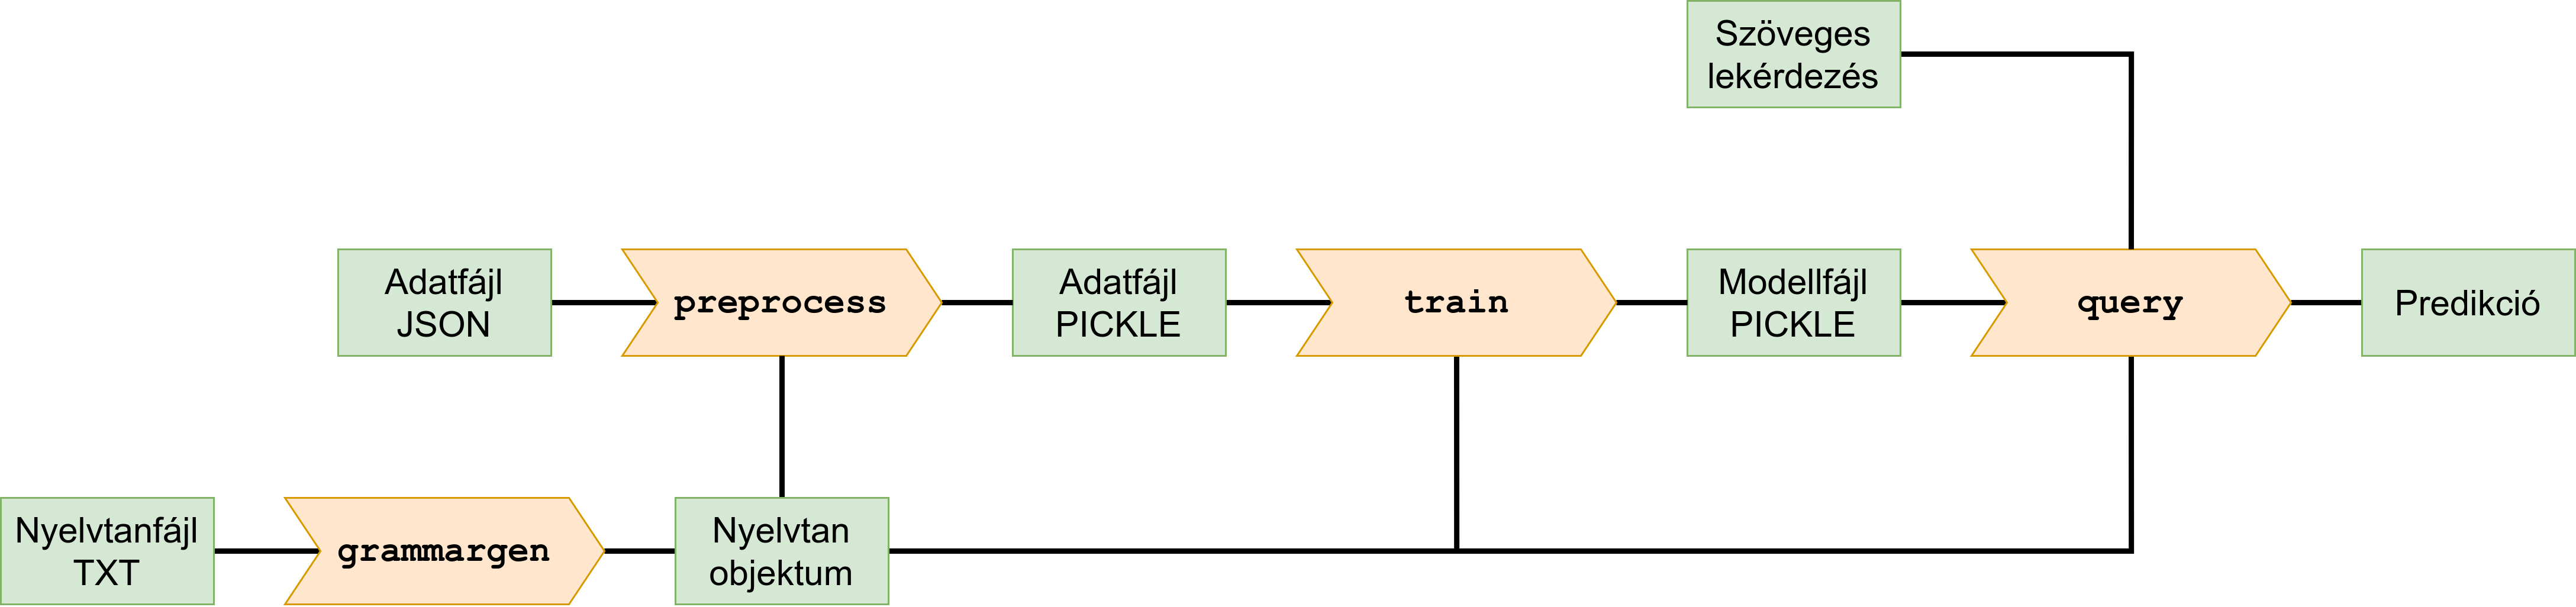
\includegraphics[width=\graphicswidth]{munkafolyamat.png}
  \caption{A SASN munkafolyamatai}
\end{figure}

A szoftver tetszőleges adathalmazon futtatható, nincs szükség a forráskód módosítására különböző nyelvek vagy példák használatához. Ezt a tulajdonságot a moduláris architektúra biztosítja: az összes adathalmaztól függő fájl és beállítás egy szeparált \verb|datasets| könyvtárban kerül megadásra. Mindegyik mód esetében paraméterként biztosítandó az adathalmazhoz tartozó alkönyvtár neve, hogy a SASN betölthesse az abban elhelyezett \verb|settings.py| fájl konfigurációs opcióit.

Az adathalmaz keretében definiált beállításokon túl további konfiguráció biztosítható egyszeri futás erejéig a \verb|--set| kulcsszó paraméter segítségével. Ezek a parancssori beállítások használhatók az adathalmaz keretében definiált beállítások felülírására is. Például a \verb|--set SEED=0| paraméter a randomszám-generátor "SEED" értékét írja felül, úgy, hogy az \verb|0| legyen (az MLforSE adathalmazban megadott \verb|42| helyett).

A program által értelmezhető parancsokkal kapcsolatban angol nyelvű segítség kérhető a \verb|--help| kapcsoló segítségével. Amennyiben egy adott alparancssal kapcsolatban szükséges segítség előhívása, az megtehető a parancsnév, majd a \verb|--help| kapcsoló specifikálása által.

\subsection{Nyelvi modul generálása}

A SASN központi eleme a beépített nyelvtani generátor modul. A generátor egy egyedi metanyelven megadott leírást képes feldolgozni, és az alapján egy teljes értékű parser és unparser programcsomagot előállítani.

Parser névvel illetik a fordítóprogramok szintaktikai analízis fázisát kezelő programokat. Feladatuk egy tokenszekvencia szintaxisfává történő alakítása, azaz a nyelvtan szabályainak felismerése az inputon. A tokenszekvenciát az eredeti szövegből a lexer állítja elő a lexikai analízis során. Számos fordítóprogram szétválasztja a lexikális és a szintaktikai analízis szakaszát, de lehetséges ezeket együtt is kezelni. A SASN által generált parser elkülöníti ezeket, azonban a generáláshoz nem szükséges megadni külön lexikai és szintaktikai definíciókat.

A nyelvtangenerátor nem vár a fejezet elején leírtakon túl további parancssori argumentumokat. Az adathalmaz könyvtárából importálásra kerül a beállításokat tartalmazó modul (\verb|settings.py|), amely meghatározza a további fájlok elérési útvonalait. A generátor modul először lexikális és szintaxis elemző algoritmusokkal vizsgálja meg a nyelvtanfájlt, majd a feldolgozás végeztével előállítja a nyelv szabályainak egy belső reprezentációját.

\subsection{A metanyelv}

A SASN által alkalmazott metanyelv egy olyan jelölésrendszer, amely alkalmas programozási nyelvek lexikai és szintaktikai rendszereinek leírására. A nyelvtanfájlok egyszerű szöveges fájlok, amelyek az alábbiakban leírt jelölésrendszerben tartalmazzák a szabályok definícióit valamint további nyelvi konstrukciók leírásait.

Ez a felsorolás áttekinti a legfontosabb jelöléseket és azok jelentését:

\begin{itemize}[noitemsep]
  \item \textbf{Komment}\ \ \ \ A leírások tartalmazhatnak kommenteket, melyeket a metaparser a szöveg feldolgozása során figyelmen kívül hagy. A komment kezdetét egy \verb|#| szimbólum jelöli, majd az ezután következő összes karakter az első sortörés karakterig (\verb|\n|) a komment részét képezi.
  \item \textbf{Szabály definíció}\ \ \ \ Minden definíció egy baloldali (lhs) és egy jobboldali (rhs) elemet tartalmaz, köztük egy \verb|=| karakterrel. A baloldal a szabályhoz tartozó azonosító, ezzel a névvel lehet más szabályokban hivatkozni rá. A jobboldal pedig egyike a rendelkezésre álló nyelvtani konstrukcióknak. A szabályokat mindig \verb|;| karakterek zárják.
  \item \textbf{Reguláris kifejezés}\ \ \ \ A programozási nyelv tokenjei Python-típusú reguláris kifejezésekkel \parencite{Kuca} adhatók meg. A reguláris kifejezést egyszeri (\verb|'|) vagy dupla (\verb|"|) aposztrófok közé kell elhelyezni. Az aposztrófok a reguláris kifejezésekben feloldójelek (escape-szekvenciák) segítségével jelölhetők.
  \item \textbf{Szabály referencia}\ \ \ \ A szabályokra a nevükkel lehet hivatkozni. Ekkor a hivatkozás pontján a hivatkozott szabálynak teljesülnie kell az inputra, hogy a szintaktikai elemzés folytatódhasson.
  \item \textbf{Beágyazott akció}\ \ \ \ A beágyazott akciók olyan hivatkozási pontok, amelyek előre definiált rutinokat hívnak meg, ezáltal módot adva tetszőleges elemző és transzformációs lépések végrehajtására. Az akciókra történő hivatkozás egy \verb|@| karakter után történhet az akcióhoz tartozó függvény nevének megadásával.
  \item \textbf{Beágyazott akció definíciók}\ \ \ \ A beágyazott akciók forráskódja \verb|%{| és \verb|}%| karakterek között adható meg. Ezek a blokkok Python kódot tartalmazhatnak, amelyek ad verbum kerülnek beillesztésre a parser és unparser modulok elejére. Felhasználásuk célja elsősorban a beágyazott akciókhoz tartozó függvények definiálása. A leírásokban több ilyen blokk is elhelyezhető, ezeket a metaparser sorrendtartón konkatenálja.
  \item \textbf{Szekvencia}\ \ \ \ A vesszővel elválasztott nyelvtani konstrukciók mindegyike sorban felismerésre kell kerüljön az inputon.
  \item \textbf{Rendezett opciók}\ \ \ \ A \verb=|= karakterekkel elválasztott nyelvtani konstrukciók legalább egyike felismerésre kell kerüljön az inputon. A konstrukciók sorrendje számít, azaz ha egy adott ponton több opció is teljesülne (a szabály nem felelne meg az LL(1) feltételnek), akkor az elsőként megadott szabály lesz az irányadó.
  \item \textbf{Multiplikátorok}\ \ \ \ A \verb|?|, \verb|*|, \verb|+| karakterek azt jelentik, hogy az utánuk megadott konstrukció, sorrendben, 0 vagy 1, 0 vagy tetszőleges, 1 vagy tetszőleges alkalommal ismétlődhet. Ezek az unáris operátorok prefix jelölést használnak.
  \item \textbf{Zárójelek}\ \ \ \ A nyelvtani konstrukciók kötési sorrendje befolyásolható zárójelek elhelyezésével. A nulláris (reguláris kifejezés, szabály referencia, akció referencia) és unáris (multiplikátorok, ugrás) konstrukciók precedenciája egyértelmű. Csupán két bináris operátor van, az opció és a szekvencia, melyek közül a szekvencia kötése az erősebb. Ez megváltoztatható zárójelek segítségével.
  \item \textbf{Ugrás}\ \ \ \ A \verb|>| karakterrel lehetőség van egy szabály felismerésére, anélkül, hogy az utána beépülne az előállított szintaxisfába. Programszöveg-generálás során ezek a szabályok szintúgy átugrásra kerülnek.
  \item \textbf{Térköz}\ \ \ \ A nyelvtan definiálásakor a térközöknek csak ritkán van jelentősége. Ilyen esetek a kommentek lezárásához szükséges sortörések, valamint az akciók és szabályok neveinek lezárásához használt tetszőleges térközök. Reguláris kifejezések és akció definíciók esetén a térközöket a program eredeti formájában megtartja. Más esetekben a térközök nem jelentősek, formázási célra szabadon felhasználhatók.
\end{itemize}

Ez az áttekintés főleg a nómenklatúrát hivatott bemutatni, nyelvtanfájlok írásához további segítséget az \verb|mlforse| adathalmazhoz írt Python nyelvtan definíciója nyújt. A legtöbb tekintetben a metanyelv használata megegyezik az EBNF szintaxisleíró nyelvével, így sokak számára könnyen értelmezhető és elsajátítható lehet.

A beágyazott akciókhoz megadhatók parser és unparser függvények is a \verb|parse_| és az \verb|unparse_| előtagok segítségével. Ezek a függvények kerülnek majd meghívásra amikor az elemzés során a megfelelő grammatikai konstrukciók vagy szintaxisfa csúcsok következnek. Mindkét esetben a függvények megkapják paraméterként a feldolgozás állapotát reprezentáló objektumot, amellyel szabadon rendelkezhetnek.

A parser függvények visszatérési értéke vagy egy \verb|TokenNode|, egy \verb|RhsActionNoMatch| vagy \verb|None|. Az első esetben a szabály sikeresen felismert egy terminális szimbólumot az inputban. A második esetben a szabály felismerése sikertelen volt, ekkor a \verb|msg| attribútum a bukás magyarázatául szolgál. A harmadik esetben csöndes felismerés történt, azaz a szabály sikeres volt, de nem állított elő új tokent.

Az elemző algoritmus jellegéből adódóan a sikertelen felismerés önmagában még nem jelent problémát. A 0-vagy-1, 0-vagy-több valamint az opció konstrukciók lehetőséget adnak arra, hogy egy konstrukció ne kerüljön felismerésre, de az input mégis valid legyen. Ennek kezelésére az elemző algoritmus előretekint egy szimbólumot a tokenszekvenciában (lookahead), és annak értékétől függően folytatja az elemzést. A \verb|RhsActionNoMatch| visszatérési érték pontosan ezt a célt szolgálja.

\subsection{Adathalmazok előfeldolgozása}

Egy JSON formátumú adathalmaz előfeldolgozása könnyedén elvégezhető a SASN segítségével. Az általános paramétereken túl csupán az input JSON fájl és az output bináris fájl elérési útvonalát kell megadni. Az előfeldolgozás felhasználja a beállításokban megadott \verb|PARSE| és \verb|UNPARSE| függvényeket, ezáltal ennek a végrehajtási módnak az előfeltétele a nyelvtani generálás elvégzése.

A példa adathalmaz esetében a JSON fájl formátuma megfelel a CoNaLa \parencite{Yin+18a} specifikációnak. A program minimálisan csak az \verb|intent| és a \verb|snippet| mezőket várja el, de a CoNaLa ezenkívül meghatározza a \verb|question_id| és a \verb|rewritten_intent| mezőket is. A SASN jelen formájában nem használja fel ezeket a kiegészítő információkat, a kérdéseket az előfordulásuk sorrendjével azonosítja. Az alternatív feladatleírások az eredeti adathalmaz jellegzetességéből fakadóan kerültek generálásra, ugyanis a StackOverflow\footnotemark{} weboldalról automatikus módon begyűjtött feladat-megoldás párok több megfogalmazásban is tartalmazták a kérdést feltevők eredeti intencióját.

\footnotetext{https://stackoverflow.com/}

A preprocesszált adathalmaz formátuma a Python által sztenderdizált pickle bináris protokoll \parencite{Pit18a}. A pickle protokoll használatával lehetőség nyílik Python objektumok egyszerű szerializációjára, amely alkalmassá teszi a tokenizált szövegek és a szintaxisfa-építő akciókká alakított programkódok tárolására. A reprezentáció lapos, azaz a feladat-megoldás párok egymást követik sorban a fájlban. A SASN az előfeldolgozás során mind az input mind az output esetében épít szótárakat, amiket először ír ki a fájlba, azt követve a példák számával, a szótárak leghosszabb elemeinek hosszával, majd legvégül magukkal a példákkal. A példák kiírás előtt átesnek egy véletlen keverésen is.

\subsection{Tanítás adathalmazon}

Az előfeldolgozott adathalmaz fájlok alkalmasak a SASN predikciós algoritmusaként használt mesterséges neurális háló tanítására. A \verb|train| végrehajtási mód az adathalmazt várja bemenetként, és egy betanított hálót produkál kimenetként. A mód invokációjakor ezen komponensek fájlrendszerbeli útvonalát várja parancssori paraméterként. A tanítás végeredménye egy pickle formátumú PyTorch modell objektum.

Fontos megjegyezni, hogy a tanítás - az alkalmazott modelltől függően - akár nagyon sok időt is igénybe vehet. Különösen fontos lehet odafigyelni ilyenkor a példák számára és bonyolultságára, valamint a \verb|MAX_EPOCH| beállítás értékére.

\subsection{Lekérdezés}

A lekérdezés a Bevezetésben leírtakhoz hűen két paramétert vár: az egyik a feladat leírása (\verb|query|), a másik a döntéshozatalhoz szükséges szabályrendszer. Utóbbi egyrészt a betanított modellből (\verb|model|), másrészt a beállítások között megadott nyelvtanfájlból áll. A lekérdezés eredménye a legjobb valószínűséget elérő program egyik reprezentációja. Amennyiben a reprezentáció szintaxishelyes, akkor a végeredmény a programszöveg, ha nem, akkor szintaxisfa-építő lépések sorozata.

\section{Hibaüzenetek és magyarázataik}

A SASN három típusú hibaüzenetet küldhet:

\begin{itemize}[noitemsep]
  \item \textbf{GrammarError} : Ilyen hibák a nyelvtani leírások elemzése során fordulhatnak elő. A hiba üzenete mindig leírja annak pontos okát és pozícióját is.
    \begin{itemize}[noitemsep]
      \item Lexikai hiba: A fájl vagy egy invalid karaktert, vagy egy befejeztlen sztringet, esetleg egy befejezetlen definíciós blokkot tartalmaz.
      \item Szintaktikai hiba: Az egyik felismert karaktersorozat olyan tokent alkot, amely nem megengedett a metanyelvtan szerint.
      \item Szemantikai hiba: A nyelvtan nem engedélyezi bal-rekurzív szabályok alkalmazását, ezért amennyiben ilyet észlel, azonnal terminál. Szemantikai hiba léphet fel akkor is, ha olyan beágyazott akcióra vagy szabályra történik hivatkozás, amelyhez nem tartozik definíció.
    \end{itemize}
  \item \textbf{LanguageError} : Ezek a nyelvi hibák nem a nyelvtanfájl, hanem a programszövegek analízise során lépnek fel, és hasonló okokból kifolyólag, mint a GrammarError lexikai és szintaktikai hibái.
  \item \textbf{SettingNotFoundError} : Ezek a hibák arra figyelmeztetnek, ha az adathalmaz elkészítésekor nem minden SASN által igényelt beállítás került specifikációra.
\end{itemize}

A fent leírt hibákon túl a SASN néha figyelmeztetéseket is küld. Ezek vagy potenciálisan hibás viselkedést jeleznek, vagy optimalizálási lehetőségeket javasolnak. Az utóbbira példát jelent az üres vagy egyelemű szekvencia vagy opció konstrukciók, valamint a fölösleges ugrás, 0-vagy-1, 0-vagy-több, 1-vagy-több multiplikátorok jelenlétére való felhívás is. Ezeket a hibákat a log üzenetek között jeleníti meg a program.

\section{A program leállítása}

A konténer előterében futó alkalmazás háttérbe küldhető a \verb|Ctrl + Z| billentyűkombinációval. Ez megszakítja a program futását, amelyet a előtérben folytatni az \verb|fg| paranccsal lehet. A konténer előterében futó alkalmazás megállítható a \verb|Ctrl + C| billentyűkombinációval. Háttérben futó alkalmazások megállításához a \verb|kill| parancs használható. Az interaktívan futó konténer egyed leválaszható a szülő shell munkamenetről a Docker kilépési szekvencia (\verb|Ctrl + P| után \verb|Ctrl + Q|) bevitelével. A leválaszott munkamenet hasonlóan folytatható, mint ahogyan egy nem-interaktívan indított konténerbe lehet becsatlakozni. A konténer leállítása történhet az összes csatlakoztatott interaktív munkamenet megszüntetésével, vagy a \verb|docker stop sasn| paranccsal, ahol \verb|sasn| a leállítani kívánt konténer neve.

\section{Eltávolítási útmutató}

Mivel a futtatás Docker-virtualizált konténereken keresztül történik, minden adat és ideiglenes fájl egy izolált közegben kerül létrehozásra, ezáltal a Docker által kezelt állományokon kívül más melléktermék nem keletkezik. Ezek eltávolítása megszokott Docker parancsokkal lehetséges.

A program eltávolítása előtt le kell állítani minden SASN-t futtató konténert. Amennyiben egy konténer az \verb|--rm| kapcsoló nélkül lett elindítva, annak tartalma leállítás után is jelen van a fájlrendszerben. A \verb|docker container prune| parancs használható a nem futó konténerek eltávolítására. A \verb|docker image prune -a| parancs eltávolítja a konténerrel nem rendelkező konténerképeket, beleértve az ideiglenes fordítási rétegeket is. Egyéb objektumok törlésére nincs szükség, mivel a program nem példányosít vagy igényel hálózatokat (network) vagy köteteket (volume).

Fontos megjegyezni, hogy a szoftver eltávolítása csak akkor tekinthető teljesnek, ha a dokumentáció és a forráskód is törlésre került, hiszen ezekre ugyanazok a licenszfeltételek vonatkoznak, és ugyanúgy részét képezik a teljes programnak, mint a futtatható állományok. Ez kiterjed a rendszer egészére, beleértve a biztonsági mentéseket, gyorsítótárakat, fájlrendszer-szemetest, legyen szó akár a szoftver egészéről, akár részleteiről.

\chapter{Fejlesztői dokumentáció}

A fejlesztői dokumentáció azon programozók számára íródott, akik szeretnék megérteni a SASN működését, vagy esetleg módosításokat is szeretnének végezni rajta. Bemutatja a program általános szerkezetetét valamint az implementáció főbb aspektusait. A dokumentáció feltételez középhaladó szintű jártasságot a felhasznált fejlesztői eszközök és technológiák terén, nem célja azok alapvető működésének bemutatása.

A program használatáról a felhasználói dokumentáció számol be, az ott leírtakat fontos fejlesztés közben is figyelembe venni. Mivel a SASN főleg szakirányi ismeretekkel rendelkező informatikusok számára bizonyulhat hasznosnak, ezért már a felhasználói dokumentáció is tartalmaz bizonyos implementációs részleteket, különösen a nyelvtanfájlok kezelésével kapcsolatban.

\section{Fejlesztői ismertető}

A tény, hogy a szoftver egy Docker konténerként kerül disztribúcióra nagyban segít nem csupán a felhasználói, de a fejlesztői függőségek kezelésében is. Ennek következtében a fejlesztői környezet nem tér el nagy mértékben a felhasználói környezettől. Minden felhasználói függőség egyben fejlesztői függőség is. A forráskód verziókezelése git segítségével történik, míg a kódbázist a \verb|https://github.com/dinatamas/sasn| publikus GitHub repository tárolja. Ez lehetővé teszi a széleskörű kollaborációt és a forráskódhoz való egyszerű hozzáférést.

A szoftver szinte teljes egésze a Python 3.8 programozási nyelven íródott, a PyTorch\footnotemark{} machine learning framework alapjain. Ezen kívül csak kevés további dependencia szolgáltatásait veszi igénybe. Az NLTK \parencite{BKL09a} természetes nyelvekkel foglalkozó könyvtárat a bemenet felbontására, a tqdm\footnotemark{} modult az előfeldolgozás és tanítás állapotának konzolos megjelenítésére használja. Szükség esetén (például a licensz feltételek miatt) mindkét modul könnyedén eltávolítható. Implicit módon további nem sztenderd könyvtárak is felhasználásra kerülnek, mint például a \verb|numpy| elnevezésű matematikai programcsomag\footnotemark{}, azonban ezek magának a PyTorch-nak is az előfeltételei, ezért a helyettesítésük számos problémával járhat.

\footnotetext{https://pytorch.org/}
\footnotetext{https://github.com/tqdm/tqdm}
\footnotetext{https://numpy.org/}

Rövid megjegyzést érdemelnek a fejlesztői dokumentációban elhelyezett UML diagramok. Mivel az implementáció Python nyelven történt, az UML diagramok számos jellemzője kevésbé érvényesül, mint például a C++ vagy Java nyelveken tudna. A Python nyelv nem követeli meg a típushelyességet, ezáltal a diagramokban meghatározott típusok is csak megközelítőek, és további lehetséges esetek is előfordulhatnak. Bizonyos esetekben ebből kifolyólag a típusok jelzése el is maradt. További fontos eltérés, hogy a Python nem különözteti meg a láthatóság private, protected és public szintjeit, minden attribútum és metódus publikus. A diagramok megtekintése során észben kell tartani, hogy a Python objektumok rendelkeznek alapértelmezett metódusokkal, melyeket általában csak akkor szokás feltüntetni, ha azok felüldefiniálásra kerültek. A Python nyelv nem valósítja meg az interfész, a virtuális függvény, a konstans attribútumok és metódusok fogalmait sem, sőt, az objektumokhoz akár futási időben is hozzákapcsolhatók további attribútumok és metódusok. Ez azt jelenti, hogy az UML diagramok statikus ábrái nem feltétlenül képesek a program szerkezetét bemutatni annak teljes élettartama alatt.

\section{Rendszerarchitektúra}

A SASN szerkezete és működése egy csomagdiagram segítségével szemléltethető legjobban. Két fő egysége van: az adathalmazokat tartalmazó \verb|datasets| modul, és a központi \verb|sasn| modul. Ezutóbbi univerzális funkciókat lát el, míg az előbbi modulárisan cserélhető részeket tartalmaz. Az egységek fő kapcsolódási pontja a \verb|main| csomag és az adathalmazok \verb|settings| csomagjai között jön létre. Futtatáskor egy parancssori argumentum segítségével futási időben kerül a főprogram konfigurálásra a beállításokat tartalmazó fájl alapján. Mindent, ami az adott adathalmazhoz tartozik, a program a \verb|settings| fájl alapján ér el, míg minden főprogrambeli kód a \verb|main| belépési ponton keresztül kerül végrehajtásra.

\begin{figure}[H]
  \centering
  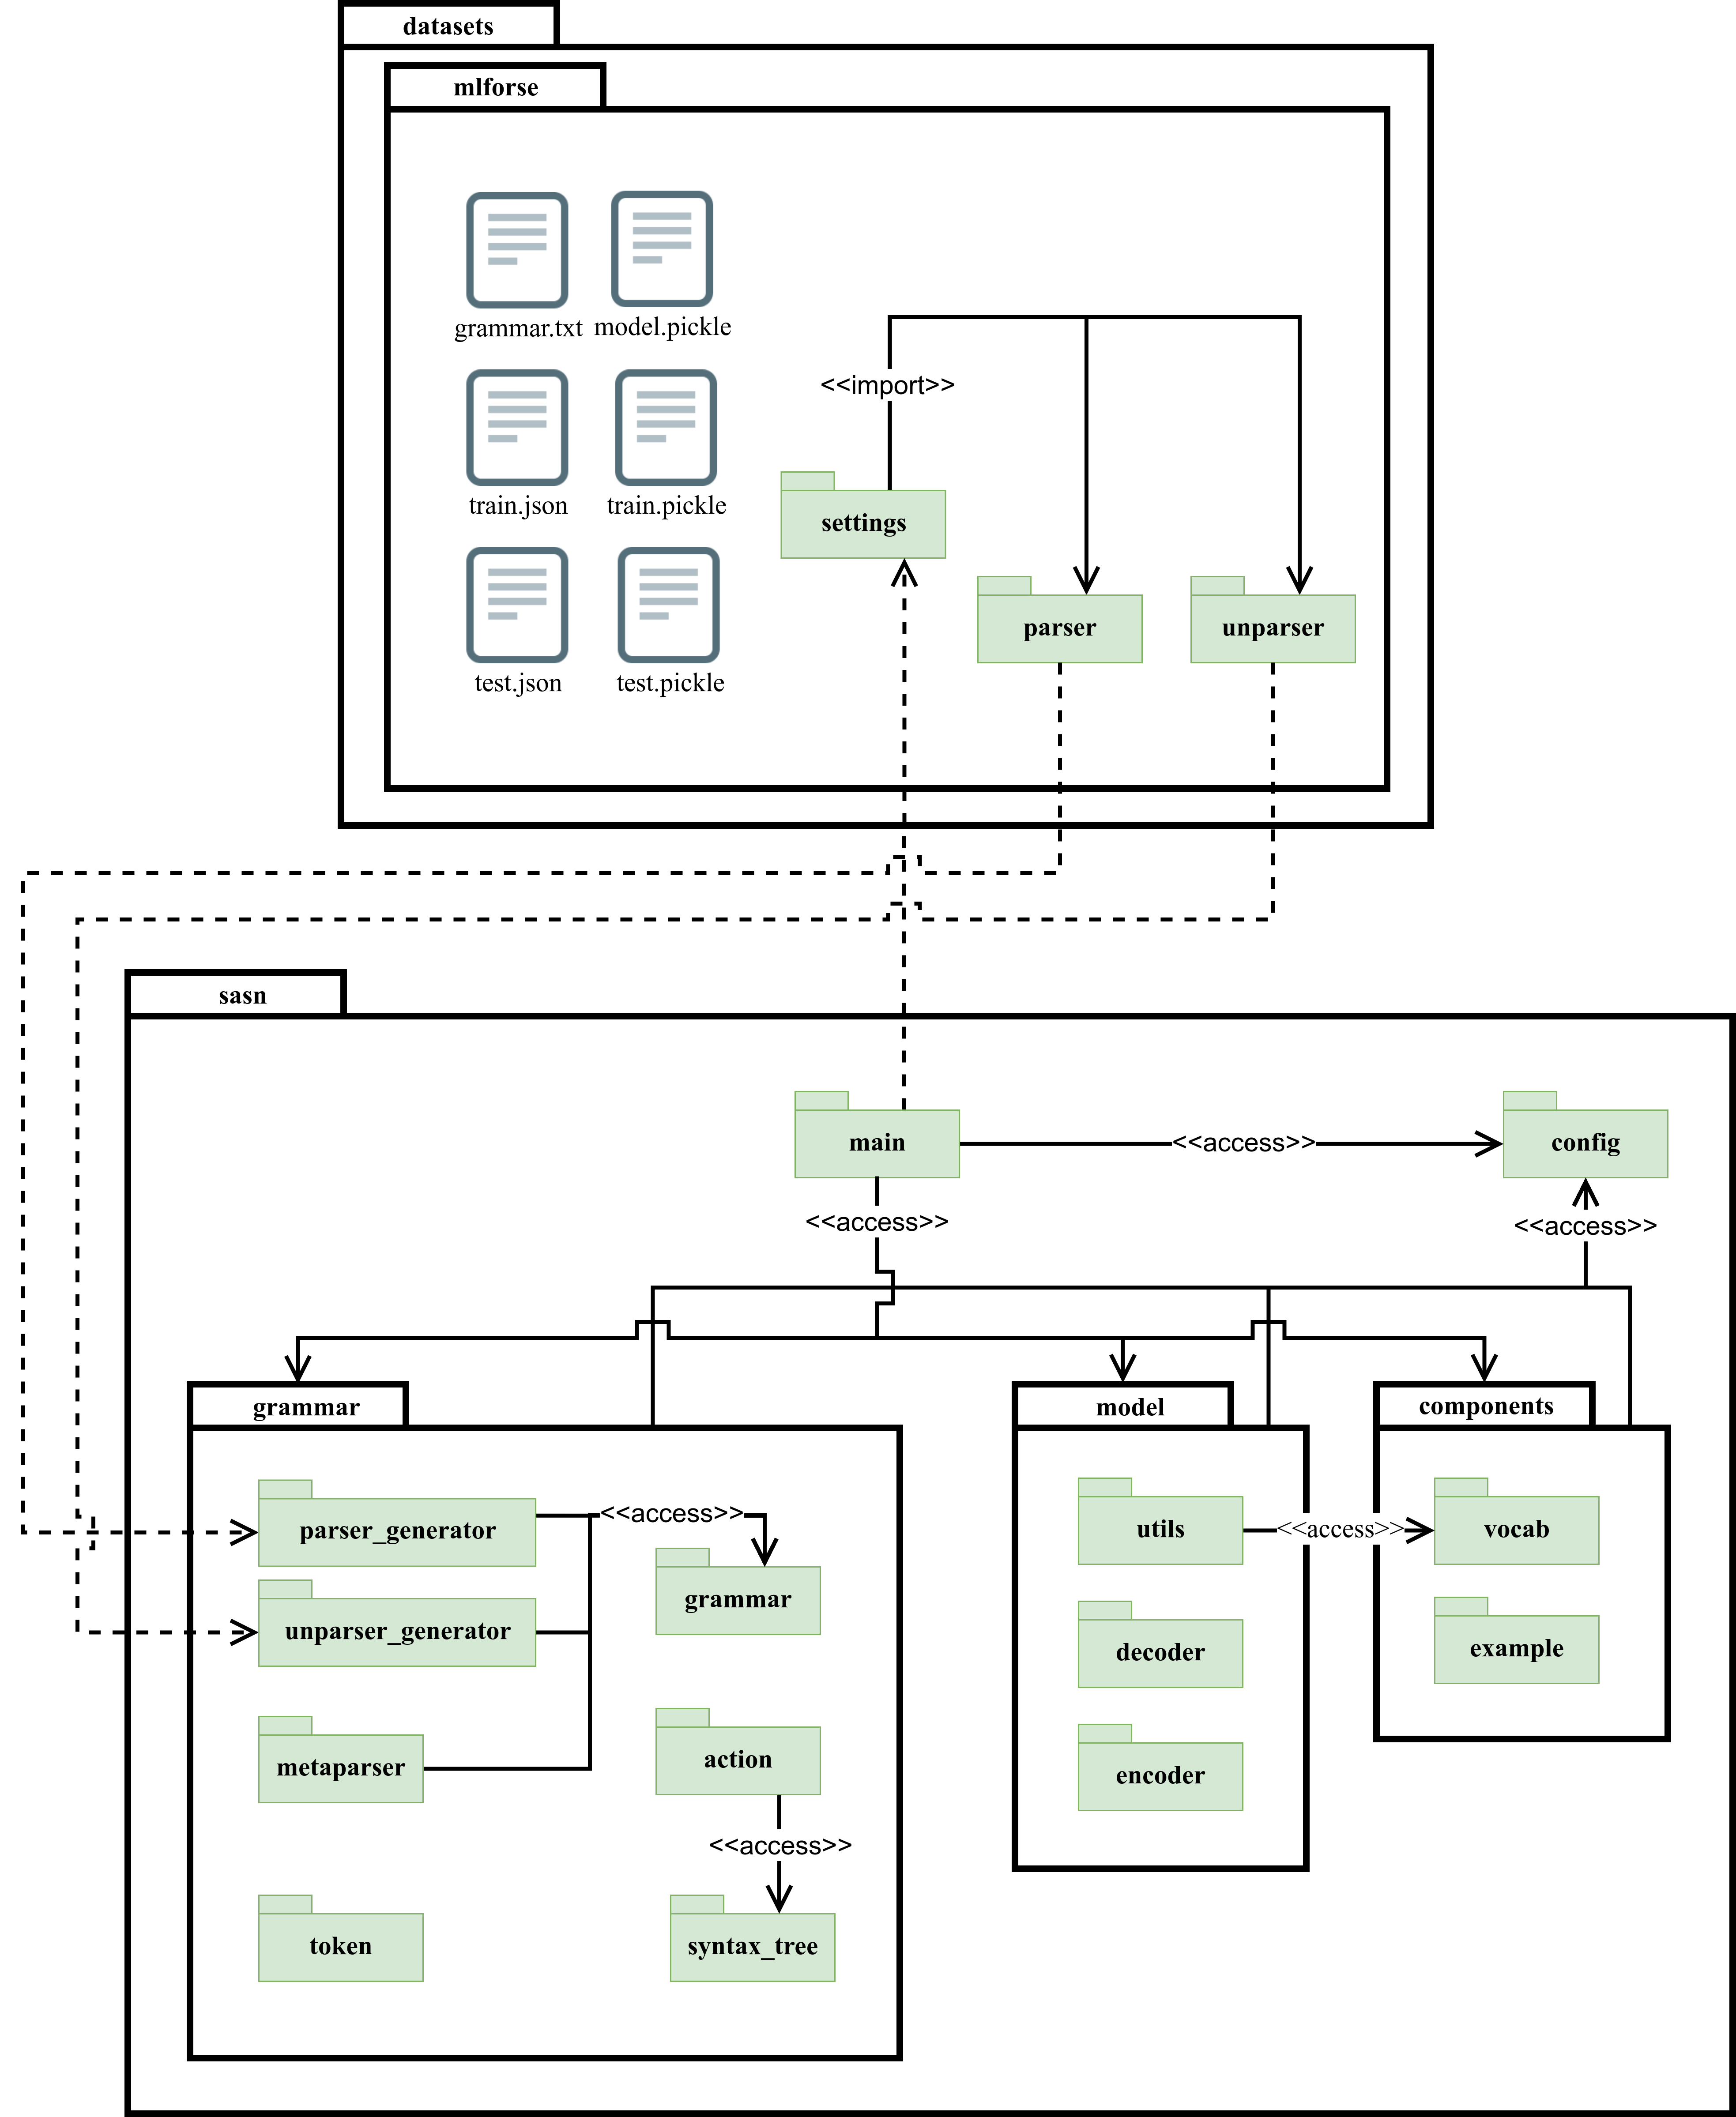
\includegraphics[width=\graphicswidth]{csomagdiagram.png}
  \caption{Bővített csomagdiagram}
\end{figure}

Egy másodlagos kapcsolódási pont is létrejön a két egység között. Az adathalmazzal való munkához nem szükséges a nyelvtani transzformációk elvégzésére szolgáló programok biztosítása (bár ez is lehetséges), hanem elegendő egy szöveges nyelvtan specifikációja, amely alapján a SASN képes automatikusan legenerálni a transzformációs modulokat. Az \verb|mlforse| adathalmaz erre a mechanizmusra épít, így tulajdonképpen egy függőségi kapcsolat áll fenn a parser és unparser, valamint a generátoraik között. Ez a generálási dependencia nem része a csomagdiagramok klasszikus jelölésrendszerének, de annyira központi eleme a SASN szerkezetének, hogy az ábrán szaggatott vonallal mégis jelölésre kerül.

A csomagdiagram bemutatja az alrendszerek főbb belső szerkezetét is. Az adathalmazok legfontosabb modulja, amely minden adathalmaz-specifikus elemet összefog, a \verb|settings.py| fájl. Ez tartalmazza konfigurációs paraméterként az összes adatfájl és a generált komponensek elérhetőségét. Az áttekinthetőség érdekében ezek az adatfájlok is fel vannak tüntetve ikonokkal.

\section{Az implementáció ismertetése}

\subsection{Főprogram}

A szoftver belépési pontja a \verb|main.py| modulban található. Itt a legfontosabb inicializáló lépések kerülnek végrehajtásra. Fontos megjegyezni, hogy a Python import rendszere miatt nem ez az első hely, ahol kód kerülhet végrehajtásra, ugyanis minden importált dependencia végrehajthat tetszőleges utasításokat annak érdekében, hogy a globális névterébe minden szükséges értéket felvegyen.

A főprogram első feladata a parancssori argumentumok értelmezése, amit a sztenderd könyvtárbeli \verb|argparse| modul segítségével tesz meg. Klasszikus megoldásként a modul nyújtotta "subparser" funckionalitást lehet kihasználni a többszintes alkalmazás felületének leírására. A \verb|config_parser| elemző az összes alparancs által használt közös paramétereket fogja össze.

Az \verb|increase_subcommand_max_position| függvény használatára egy ismert CPython hiba (bpo-25297) korrigálásához van szükség. A probléma alparancsok használatakor merül fel, és amennyiben a program túl hosszú neveket használ a parancssori opciók leírására, akkor bizonyos tördelési hibákat okozhat. Ennek megoldására egy kézzel számított tördelési érték kerül beállításra, amelyet frissíteni kell, amennyiben változás állt be a program konzolos interfészében.

A paraméterek feldolgozása után a konfigurációk előkészítése következik. Először a paraméterként megadott fájlból betöltésre kerülnek az adathalmaz által biztosított alapértelmezett értékek, majd ezek kerülnek kiegészítésre és felülírásra a további paraméterek által.

\begin{figure}[H]
  \centering
  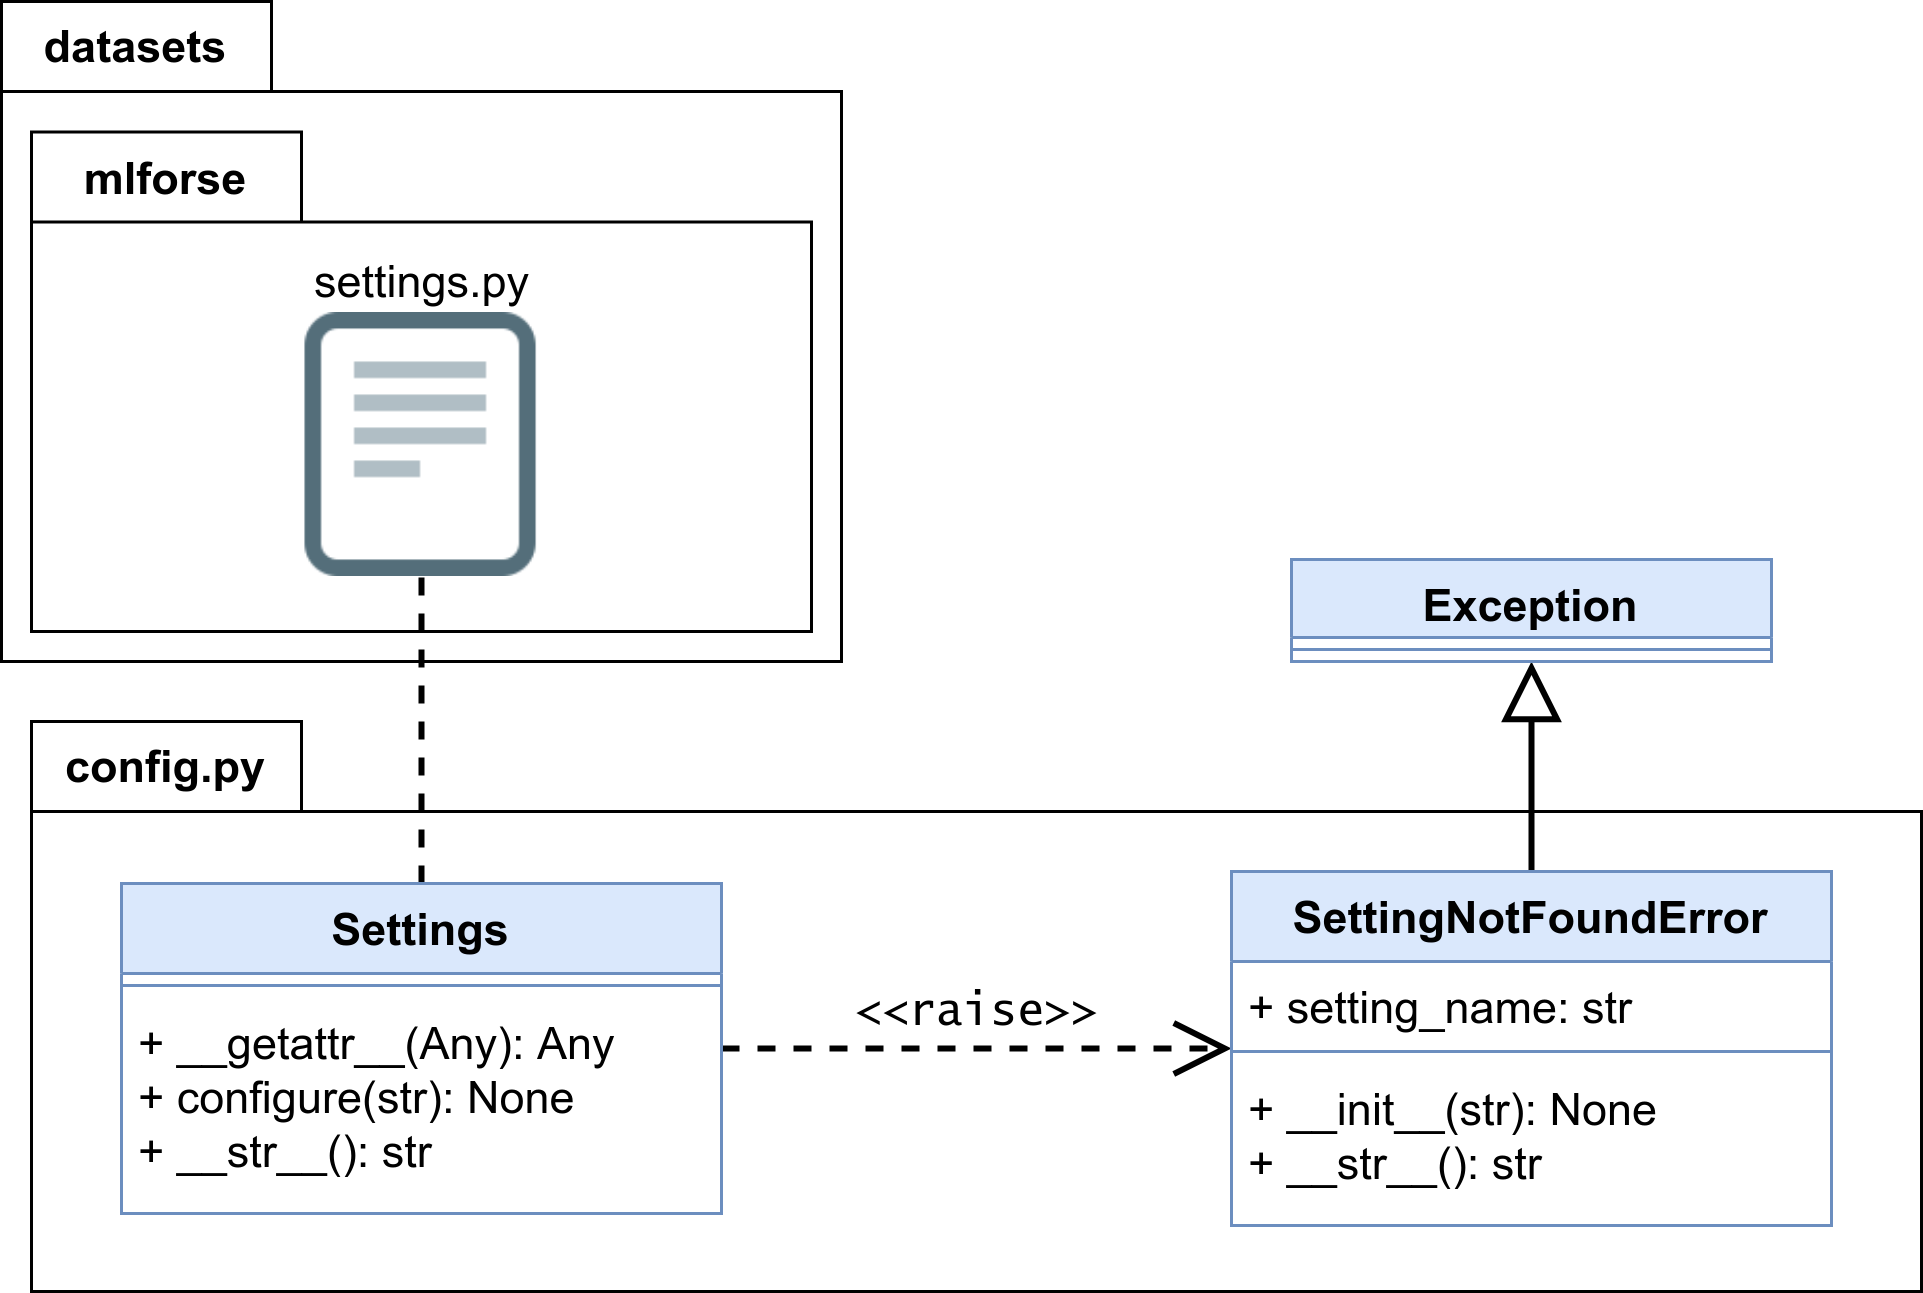
\includegraphics[width=\graphicswidth]{osztaly-diagram-konfiguracio.png}
  \caption{Konfigurációmenedzsment}
\end{figure}

A paraméterek feldolgozása majd a beállítások kezelése előfeltétele a logging motor elindításának, de érdemes - amint ezek teljesültek - inicializálni a felhasználóval történő kommunikációt. Ez segít a fellépő problémák kommunikációjában már a program végrehajtásának kezdeti szakaszában is. Amennyiben eddig sikeres volt minden lépés, a logfájlba a \verb|SASN started.| üzenet kerül kiírásra. Debugging és reprodukálhatósági célból a beállítások értékei is kiírásra kerülnek már ezen a ponton.

Az utolsó, minden végrehajtási mód esetén releváns kódelem a véletlenszám-generátor inicializációja. Ez több esetben is szükséges, mivel mind a sztenderd könyvtár, mind a \verb|numpy| és a PyTorch külön generátorokat alkalmaz. Annak érdekében, hogy a végrehajtás determinisztikus legyen a CUDA-t használó környezetekben is, bizonyos beállítások megadására van szükség \parencite{Tora}. Figyelemmel kell tartani, hogy a determinisztikus végrehajtás lassabb, mint azok a futtatások, amikor a backend nem törekszik erre. A teljesítményt csökkentő beállítások a \verb|deterministic| flag segítségével aktiválhatók. A \verb|benchmark| flag azt a viselkedést befolyásolja, hogy a CUDA alkalmazzon-e az adott környezetre mért esetleges optimalizálási technikákat. Többszörös végrehajtás esetén a backend képes felmérni, hogy milyen módokon tud az adott hardver adta lehetőségeket kihasználva időt nyerni, ezért ez a technika is nemdeterminisztikus elemeket vezethet be.

Ezen a ponton a kód elágaz a legfőbb részegységek saját alprogramjainak belépési pontjaira, amelyek mind a \verb|main.py| egy-egy függvényeként kerültek definícióra.

\subsection{Metanyelvtan modul}

A \verb|grammar| mappában található kódfájlok két fő csoportra oszthatók. Egyrészt ott találhatók a köztes jelentésreprezentációk implementációs fájljai (\verb|token.py|, \verb|syntax_tree.py|, \verb|action.py|), másrészt az ezek közötti konverziók is. A szintaxisfák és az akciók közötti átalakítások a definíciós fájljaikban találhatók, míg a szöveg és szintaxisfa közötti kétirányú konverzió olyan bonyolult feladat, hogy külön programegységeket igényel. Ezek a programegységek a nyelvtan alapján generált parser és unparser modulok.

A nyelvtan generálásakor a főprogram elsőként a metaparsert hívja meg a beállításokban specifikált nyelvtanfájlra. A nyelvtanfájl feldolgozásának két fő lépése van: a lexing majd a parsing. Ez követi egy egyszerűbb postprocessing lépés is.

A lexing lépés \verb|MetaToken| objektumokat hoz létre, amelyek eltárolják a felismert elemek típusát, sztring értékét és pozícióját is. A felismerés a \verb|MetaLexer| objektum \verb|regexs| attribútumában definiált reguláris kifejezések segítéségével történik. Minden reguláris kifejezéshez tartozik egy token elnevezés és egy előfordított Python \verb|re| objektum. Az előfordítás a teljesítménynövelés célját szolgálja. A \verb|lex| metódus sorban tekinti végig a nyelvtanfájl karaktereit, mindig ráillesztve az összes reguláris kifejezést, és az illeszkedők közül a leghosszabbat választja ki. Ez a viselkedés hasonlít a GNU lex program által alkalmazott módszerre is. Az azonos hossz mellett egyező kifejezések közül az nyer precedenciát, amelyik korábban kerül definiálásra. Igaz, megjegyzendő, hogy a metanyelvtan lexikális egységei kölcsönösen kizáró FIRST halmazokkal rendelkeznek, ezáltal minden karaktersorozatra legfeljebb egy egyező kifejezés létezik. A felismert sztringek további feldolgozáson is átesnek, például a térköz és komment metatokenek nem produkálnak token objektumot.

\vspace{0.5cm}
\begin{figure}[H]
  \centering
  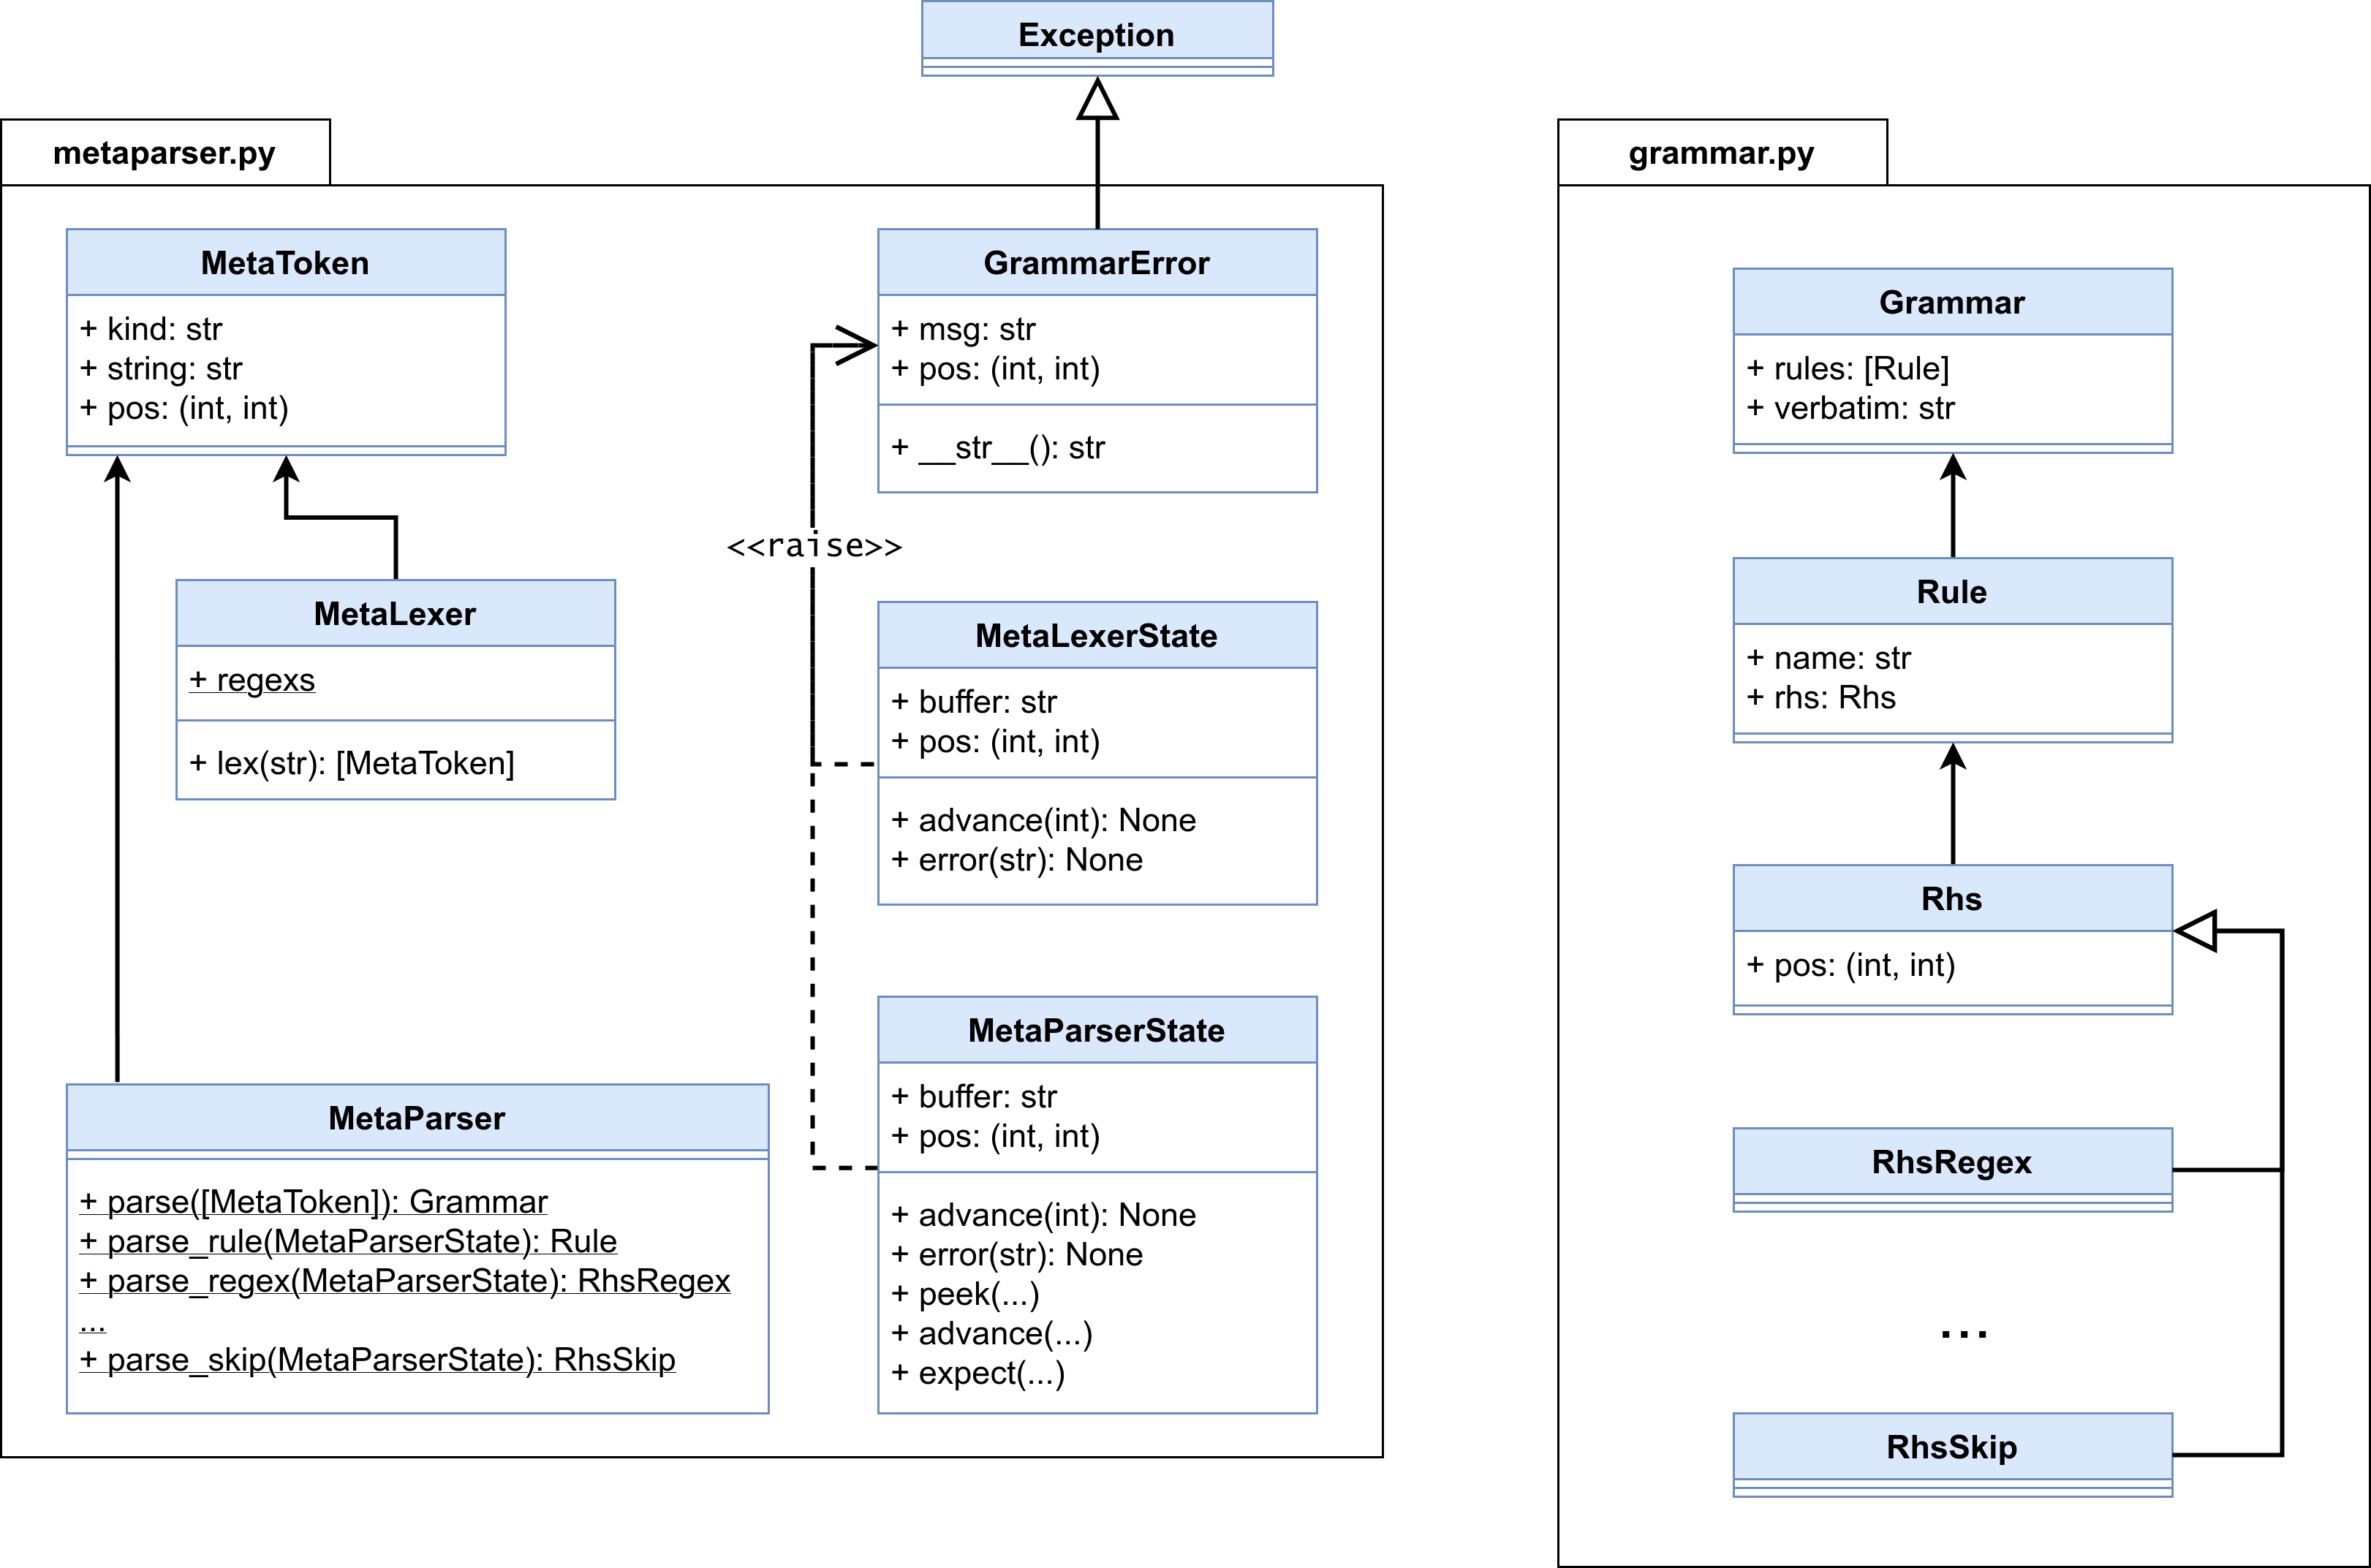
\includegraphics[width=\graphicswidth]{osztaly-diagram-metanyelvtan.png}
  \caption{A SASN grammatikai eszköztárának szerkezete}
\end{figure}

A SASN számos ponton alkalmazza azt a megközelítést, hogy külön osztályba szervezi ki a feldolgozó algoritmusok állapotát (state). Erre azért kerül sor, mert szoftvertechnológiai szempontból előnyös lehet az ilyen módon történő szeparáció. Például segíti a párhuzamosítást, valamint az elemzéshez szükséges objektumok élettartamának meghatározását is. Ez a technika hasonlít ahhoz, ahogyan például a C nyelven kerülne implementációra egy ehhez hasonló algoritmus: egy struct típus (rekord adatszerkezet) tartalmazná a feldolgozás állapotát, míg a modul névterében definiált függvények foglalkoznak az állapotátmenetekkel és a mutációkkal. A Python adta lehetőségekkel az adatelemek mellett az azokon végrehajtható állapotátmenetek is kiszervezésre kerülhetnek, ezáltal a parser függvényeknek nem az állapot attribútumaival kell szabadon foglalkozniuk, hanem meghatározott módon, a publikus interfészen keresztül léphetnek interakcióba. A függvények nem egy globális névtérben, hanem a \verb|MetaParser| osztály statikus metódusaiként kerülnek implementációra, ezáltal jobban szeparálhatók a referenciák és konzisztens marad a névtérhasználat.

A szintaktikai elemzés belépési pontja a \verb|MetaParser| osztály \verb|parse| metódusa. Ez egy metatoken szekvenciát vár paraméterül, és az egyes tokeneket a hozzá tartozó konstrukció-specifikus elemzőfüggvényekhez továbbítja. A fő metódus egyrészt szabálydefiníciókat, másrészt verbatim kódblokkokat (beágyazott akció definíciókat) dolgoz fel. Ezeken belül a specifikusabb elemzőfüggvények végzik el a feldolgozást.

Az elemzőalgoritmus egy klasszikus rekurzív leszállás elemző (recursive descent), azaz rendelkezik a tokenek felismeréséhez használható \verb|peek| (előtekintés), \verb|accept| (lehetséges elfogadás) és \verb|except| (kötelező elfogadás) metódusokkal. Ezek egy token előfeldolgozásával (LL(1) lookahead) képesek egy vagy több potenciális token elfogadására. A feldolgozó függvények ezek segítségével képesek az állapot módosítására. A metanyelvtan kifejezetten úgy lett kialakítva, hogy a parser backtracking nélkül is képes legyen feldolgozni, azaz tulajdonképpen a \verb|MetaParser| egy nagy hatékonyságú prediktív elemző, mivel a parser algoritmusok ezen osztálya az LL(k) nyelvosztály elemeit képes lineáris időben felismerni.

A szintaktikai elemzés végterméke egy \verb|Grammar| objektum, amely képes a különböző \verb|Rhs| osztályok segítségével leírni az eredeti nyelvtan tartalmát. A \verb|grammar.py| tartalma nem kerül UML diagram keretében részletesen bemutatásra, mivel rengeteg benne a különböző Rhs típusokból fakadó ismétlődés. Ez kiterjed mind magukra az osztálydefiníciókra, mind a különböző visitor osztályokban definiált metódusokra is.

A feldolgozott nyelvtanon különböző elemző függvények futtathatók. Ezek a \verb|check_grammar| és \verb|print_grammar| belépési pontokon érhetők el, de a funkciókat magukat inkább a visitor osztályok (\verb|GrammarCheckVisitor|, \verb|GrammarPrintVisitor|) valósítják meg. Ezek egy közös ősosztályból, a \verb|GrammarCheckVisitor|-ból származnak le, amely egy általános \verb|visit| metódust biztosít. Ennek a megvalósításnak az a célja, hogy a látogató metódusok ezzel az egyszerű elérési ponttal legyenek képesek meghívni a megfelelő részprogramokat. Ezt a technikát alkalmazza több, a CPython sztenderd könyvtárában AST-kel foglalkozó modul is.

A látogató osztályok is kiszervezik az aktuális állapotukat, ezzel lehetővé téve, hogy egyetlen látogató példány több párhuzamos látogatást is lefolytasson. A \verb|GrammarVisitorBase| nem csupán a fent leírt két osztály egységesítésére szolgál, hanem hozzájuk hasonló további látogatók definíciójára is lehetőséget ad. Ehhez szükséges egy általános \verb|Grammar|-szintű belépési pont biztosítása, majd utána az összes \verb|Rule| és \verb|Rhs| osztályhoz egy látogatási metódus implementációja. Ezzel lehetővé válik a teljes nyelvtant reprezentáló fa bejárása. A kiszervezett állapot technikájának alkalmazása természetesen nem kötelező, csak ajánlott. Az ősosztály biztosít egy \verb|visit_wrapper| függvényt is, amely felülírásával lehetővé válik még pontosabb felügyelet szerzése a fa látogatásának módjával kapcsolatban. Ez kihasználásra kerül például a \verb|GrammarPrintVisitor| esetében, ahol a vizitációk előtt és után szükséges az indentáció kezelése, annak érdekében, hogy még olvashatóbb legyen a nyelvtan sztring reprezentációja.

A főprogram a nyelvtani generálás során egyrészt kiírja a nyelvtan szerkezetét, másrészt le is ellenőzi azt. Az előbbi csak akkor jut el a végfelhasználóhoz, ha a beállított log szint elfogadja a \verb|DEBUG| üzeneteket. A nyelvtan helyessége az előfeltétele minden további tevékenységnek. Az ellenőrzés szintúgy a \verb|grammar.py| fájlban definiált függvények segítségével történik: például a \verb|leftmost_rules| szubrutin képes megállapítani, hogy egy adott szabályban előfordul-e balrekurzió. Ehhez felépít egy \verb|cv_cache| elnevezésű gyorsítótárat, amelyben azt tárolja el, hogy az egyes szabályok eltűnhetnek-e, azaz redukálódhatnak-e epszilonná. Ez azért fontos, mert ha egy szabály eltűnhet, akkor az annak jobboldalán álló következő szabály is okozhat balrekurziót. A \verb|parents| lista a már meglátogatott \verb|Rhs| objektumokat gyűjti: ha tényleg lenne balrekurzió a nyelvtanban, akkor annak preorder bejárása (amit maga a \verb|leftmost_rules| függvény is tesz) végtelen ciklusba kerülhet. Ennek a listának a segítségével gyorsan felismerhetővé válik ez a fajta viselkedés.

A nyelvtani modul további általános eszközöket is nyújt. A \verb|can_vanish| függvényt egyrészt felhasználja maga a \verb|leftmost_rules| is, de ezen kívül fontos eleme a FIRST halmaz kalkulációját elvégző \verb|first_set| függvénynek is. Itt érdemes felhívni a figyelmet a \verb|can_vanish| és \verb|will_vanish| függvények közötti különbségre. A \verb|can_vanish| azt ellenőrzi, hogy egy szabály redukálódhat-e potenciálisan epszilonná, a \verb|will_vanish| azt, hogy mindenképpen megteszi-e azt.

\subsection{Célnyelvtan modul}

A célnyelvi modulok, azaz a generált \verb|parser| és \verb|unparser| modulok nagyon hasonlítanak a \verb|metaparser.py| példáján keresztül bemutatott nyelvi feldolgozási programokra. A bonyolultságuk abban rejlik, hogy nem egy konkrét nyelvtanra, hanem tetszőleges nyelvtanra alkalmazhatók, ezért nem is lehet olyan könnyen átlátni, mint a \verb|metaparser| esetében, de a működési elvük megegyezik.

Az elemző komponensek előállításáért a \verb|parser_generator.py| és a \verb|unparser_generator.py| programok felelnek. Az utóbbi működési elve egyszerű, mivel az \verb|unparser| mindössze egy szintaxisfa-sétáló algoritmus, ezért "boilerplate" kód beillesztésével megoldható a feladata. A \verb|parser| előállításához már szükség van generálásra, igaz, ennek a modulnak az elejére is kerül "boilerplate" kód.

A \verb|ParserGeneratorState| és \verb|ParserGenerator| hasonló elven működnek, mint a látogató osztályok a nyelvtani modulban, azaz feldolgozzák a nyelvtant reprezentáló fákat, és minden csúcs meglátogatásakor elhelyeznek a célfájlban egy megfelelő kódrészletet. Például amikor egy opció nyelvtani konstrukció kerül feldolgozásra, akkor ez a végeredmény fájlban úgy jelenik meg, hogy if-elif-else elágazásokkal megvizsgálásra kerül az összes lehetséges opció. A generált fájlban minden szabálynak megfelel egy-egy függvény, amelyeket a benne található szabály-jobboldalak szerint tölti ki a generátot. Beszúrásra kerülnek ezen kívül a nyelvtanfájlban megadott \verb|verbatim| kódrészletek is.

\subsection{Jelentésreprezentációk}

A célnyelvtan parser modulja képes a programszöveget szintaxisfává alakítani, beillesztve egy köztes lexing lépést is, amely során az eredeti jelentéstartalmat az általa generált tokenek hordozzák. A célnyelvi tokenek típusa megegyezik a metanyelvi tokenek típusával, így az további vizsgálatot nem igényel. A szintaxisfák két típusú csúcsból állnak: a leveleket képező \verb|TokenNode| és a belső csúcsokat képező \verb|RuleNode| objektumokból. Az előbbi egyszerűen egy tokent tartalmaz, az utóbbi a levezetési szabály nevét valamint - mivel nem levélcsúcsról van szó - a gyerekcsúcsokat. Ilyen szempontból a \verb|RuleNode| értelmezhető úgy, mint ami egyszerre jelzi azt, hogy a programozási nyelv szintaxisa szerint a \verb|name| elnevezésű szabály következik (általános eset), valamint azt, hogy a vizsgált szintaxisfa ezt a szabály pontosan milyen módon, milyen részfával teljesíti (konkrét eset). A két csúcstípus közös ősosztállyal rendelkezik.

A szintaxisfák kezelésére két utility függvény is elérhető. Az egyik előállítja egy szintaxisfa sztring reprezentációját, a másik két szintaxisfa egyezését vizsgálja. Mindkét függvény egy egyszerű rekurziós séta algoritmust használ alapjául, azzal a különbséggel, hogy a printer aggregációs változókat használ az eredmény előállítására, mint a checker visszatérési értékekkel operál.

Az akciók implementációja kissé bonyolultabb, mint a szintaxisfáké, mivel az utóbbi átalakító funkció ki vannak szervezve a parser és unparser modulokba. Három típusú akció létezik: \verb|ApplyRuleAction|, \verb|ReduceAction|, \verb|GenTokenAction|. Az \verb|ApplyRuleAction| egy nem-levél csúcs beszúrását jelenti, ahol a \verb|name| attribútum a beszúrt szabály nevét tárolja el. Az akciók kezelésének módja miatt az újonnan hozzáadott node lesz a levezetés következő aktív eleme, azaz a következő akció már erre az új csúcsra fog hivatkozni. A \verb|ReduceAction| egyszerűen azt jelenti, hogy az aktuális aktív csúcshoz már nem kerül beszúrásra több gyermek, így a preorder séta által meghatározott sorrendben léptetendő a következő kifejtésre váró elem. Az akció \verb|count| attribútuma azt szabja meg, hogy hány ilyen visszalépést kell végrehajtani. A \verb|GenTokenAction| hasonlít az \verb|ApplyRuleAction| akcióhoz, csak itt egy levél csúcs kerül beszúrásra, és a név helyett a token értéke kerül eltárolásra. A preorder séta szerint következő elem ekkor nem változik.

Az akciók kezeléséhez itt is rendelkezésre van bocsátva egy kiíró és egy egyenlőség vizsgáló függvény. Ezek egy egyszerű iterációs alapra építenek, és a szintaxisfákhoz hasonlóan itt is az egyik aggregátor paramétereket, a másik visszatérési értékeket használ.

A szintaxisfák akciókká történő alakítása egy preorder bejárás keretében triviális módon megvalósítható. A fordított irány kicsit nehezebb, mivel az építés közben előállított parciális szintaxisfák kezelésére is szükség van, ezért a korábbiakban bemutatott "state" technika itt is jó szolgáltatot tesz. Az akciók által reprezentált push-reduce architektúra természetes módon elvezet egy verem használatának ötletéhez, amely segítségével figyelemmel tartható a sorrendben következő csúcs.

\subsection{A neurális háló}

A tanítás a \verb|main.py| fájlban egy központi tanító ciklus segítségével történik. A megfelelő programrészek és adatfájlok betöltése után inicializálásra kerülnek a modell komponensei. A tanító ciklus külső része a megfelelő számú epoch végrehajtásáért, a belső része pedig az egyes példák feldolgozásáért felel.

A neurális háló szerkezete két fő részre oszlik, és az implementáció tekintetében kifejezetten szorosan követi a "sztenderd" architektúrát. Az encoder komponens fogadja a tenzorrá alakított bemenetet, majd feldolgozza azt egy "rejtett" (köztes) vektor reprezentációvá. Ezt fogja a decoder komponens visszafejteni a megfelelő tokenszekvenciává.

\begin{figure}[H]
  \centering
  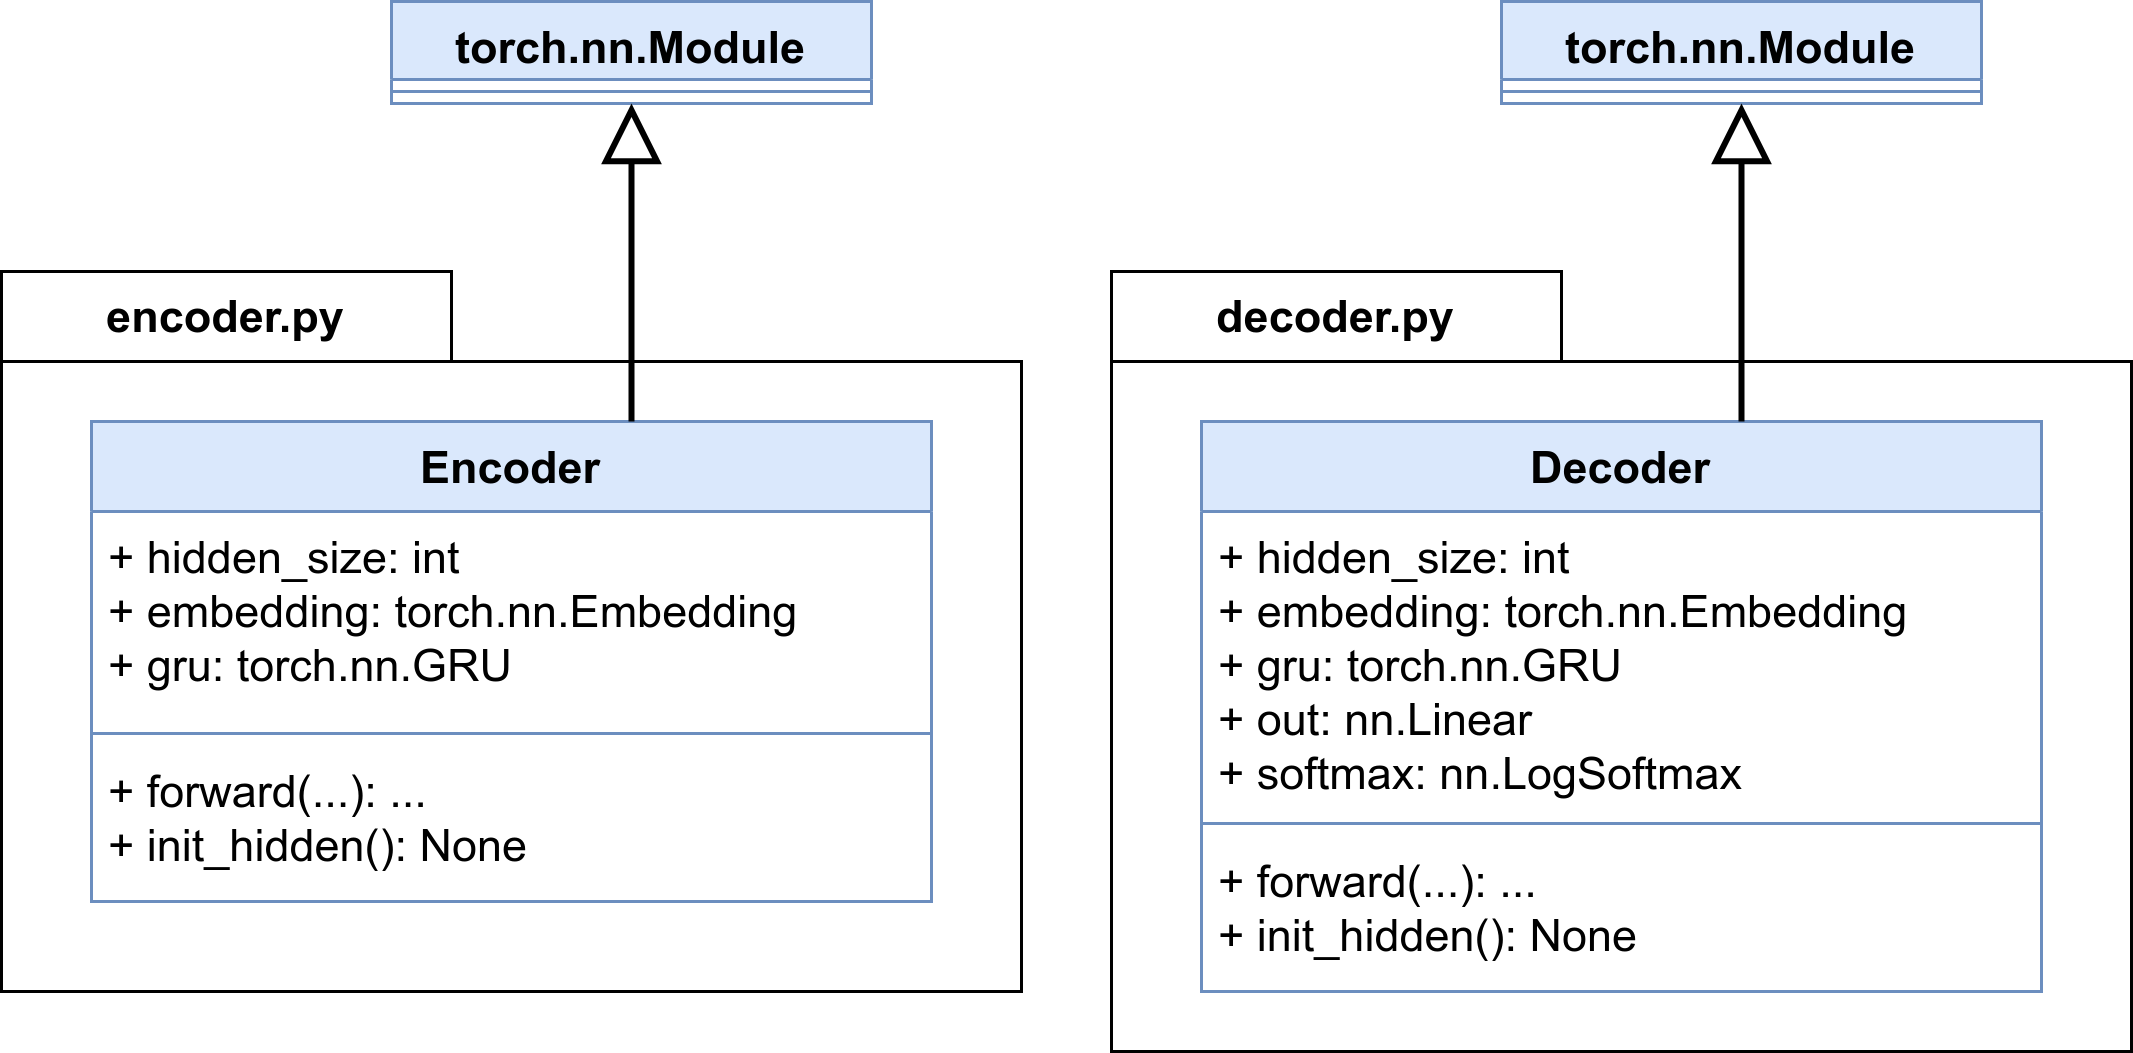
\includegraphics[width=\graphicswidth]{osztaly-diagram-modell.png}
  \caption{A neurális modell osztályai}
\end{figure}

Az encoder inicializációja az \verb|init_hidden| függvénnyel történik. Ez egyszerűen nullákkal tölti fel a rejtett vektort. Az encoder egy beágyazó réteggel és egy GRU cellával dolgozik. Az előbbi feladata a szóvektorok beágyazása, azaz a szótárbeli elemekhez valós számok rendelése. Az \verb|input_size| az összes ismert input szó száma, ez tulajdonképpen az input mérete, amikor a szavak a szótár szerinti one-hot encoding módján van reprezentálva. A one-hot encoding azt jelenti, hogy ha az adathalmaz előfeldolgozásakor 6000 különöálló szó került megjegyzésre, akkor az input egy 6000 elemes vektor, amely mindegyik adott bemenetben fel nem használt indexe 0-t tartalmaz, a felhasznált elemek pedig azonosítják az input szavakat. Az ilyen módon történő beágyazás segítéségével rengeteg memória takarítható meg. A beágyazás eredménye a kezdeti kimeneti vektor. Erre kerül alkalmazásra egy GRU egység, amely kapuk szekvenciáján vezeti keresztül a bemeneteit, és végül előállítja a teljes encoder réteg kimenetét és végső rejtett állapotát.

Az encoder eredményeire építkezik a decoder komponens. Ez is alkalmaz egy beágyazó réteget valamint egy GRU egységet, amely kimenetét egy softmax aktivációs függvényen vezeti keresztül. Ennek az aktivációs függvénynek az a szerepe, hogy a valós számvektort egy valószínűségi eloszlássá normalizálja, azaz a decoder végeredménye ennek köszönhetően felhasználható lesz a rendelkezésre álló akciók közötti valószínűségi alapon történő döntéshozatalra. A \verb|query| végrehajtási mód pontosan ezt teszi, és a legnagyobb valószínűséggel ellátott kimenetet választja ki. Ez éppen egy akció indexe lesz, amely visszafejthető a kimeneti szótár segítségével egy konkrét akcióvá. Sorozatban alkalmazva ezt a lépést éppen előállítható egy szintaxisfa-építő akciókból álló sorozat, amely éppen az elvárt végeredmény.

\section{Tesztelés}

A SASN tesztelése a dolgozat keretében biztosított \verb|mlforse| adathalmaz segítségével történik. Ez egy olyan komplexitású projekt, amely a program összes funkcióját kihasználja, ezáltal minden programelem viselkedését vizsgálja. A két fő tesztelhető aspektus a modell és a nyelvtani modul.

A modell teljesítményének elemzése, valamint általánosan véve a működésének helyessége legjobban úgy ellenőrizhető, ha példa bemenetekre adott válaszai kerülnek vizsgálatra. Ez a folyamat alkalmazható a hiperparaméterek (learning rate, hidden size, stb.) beállításának céljára is, mivel ugyan léteznek általános heurisztikák a várhatóan jó kezdőértékek megállapítására, a legcélravezetőbb megközelítés a tesztelésre alapozott döntéshozatal. A modell viselkedését több időpontban, változó számú epoch elteltével érdemes mérni. Érdemes lehet több forrásból származó példákat is tekinteni: a tanító adathalmaz egy véletlenszerű példáját, egy hasonló adathalmazból származó példát valamint egy kissé különböző, nagyobb fokú általánosítást igénylő bemenetet is a tesztelésbe vonni.

A szoftver komponensei közül legjobban a nyelvtani modul tesztelhető. A pontos eredmények érdekében az alkalmazás már tartalmaz tesztelési és verifikációs funkciókat, amelyeket az éles futás során végre is hajt, azért, hogy minden futtatási esetben garantálható legyen a helyes végrehajtás.

A köztes jelentésreprezentációk ellenőrizhetők az implementált printer függvények segítségével. Ez manuális ellenőrzéseket tesz lehetővé - az automatikus verifikáció a tranzíciós lépések segítségével végezhető. Hasznos technika az oda-vissza történő feldolgozás, amely ahhoz hasonlít, mint mikor egy angol-német fordítóprogramon ugyanazt a szöveget először angolról németre, majd az így kapott eredményt vissza németről angolra fordítják le. Ebben az esetben az ellenőrzésnek két módja van: vagy egy ismert, helyesnek feltételezett megoldás segítségével kerül összehasonlításra az eredeti bemenet és a kétszeresen fordított kimenet, vagy közvetlenül, szövegszinten történik a kiértékelés. Az utóbbi egyszerűbb, de az előbbi pontosabb tud lenni, mivel a fordítás során fellépő jelentéstartó, de nem formatartó transzformációkat is képes beleszámítani.

A Python adathalmaz esetében az automatikus ellenőrzés történhet a parse - szintaxisfa - unparse pipeline, valamint a teljes parse - szintaxisfa - akciók - szintaxisfa - unparse szekvencia szintjén is. Az egyezés autokorrekciós módszerrel ellenőrizhető a szintaxisfák között (\verb|compare_syntax_trees|) valamint a programszövegek között is. A külső forrásból történő korrekcióhoz felhasználható a Python sztenderd könyvtár \verb|ast| modulja, amellyel egy kanonizált programszöveg-reprezentáció állítható elő. Több jelentéktelen eltérés is figyelmen kívül hagyható az oda-vissza fordított sztringek között akkor, ha nem az eredeti, hanem az így kanonizált programok kerülnek összehasonlításra.

A SASN minden fent leírt tesztelési módszeren tesztelésre került, és sikerrel átment a példa Python adathalmaz esetében.

A SASN további komponensei (például a beállítások kezelésével foglalkozó kódrészletek) nem szorulnak rigorózus tesztelésre, mivel egyrészt relatíve magától értetődő az implementációjuk, másrészt a teljes munkafolyamat számos pontján kerülnek felhasználásra, ezért a többi komponensre irányuló manuális tesztelés az esetlegesen itt felmerülő hibákra is fényt derítene.

Terheléses tesztek végrehajtása is lehetséges. Az adathalmazban biztosított JSON fájlok már önmagukban is akkora méretűek, amelyek lefedik az általános felhasználói eseteket. A \verb|train.json| fájl 14'000 példa feladat-megoldás párt tartalmaz, amely egy teljesen reális méret egy ehhez hasonló feladatnál, a kézzel válogatott esetekhez képest még meg is haladja a szokásos értékeket. A szoftver kitehető nagyon nagy terhelésnek is, mint amilyet például a CoNaLa Corpus \parencite{Yin+18a} közel 600'000 példát tartalmazó gyűjteménye jelent. Az iterátor-jellegű implementációnak és az óvatos memóriakezelésnek köszönhetően azonban a SASN komplexitása lineáris a bemenet méretére, ezért ezekben az esetekben sem lesz tapasztalható hibás működés.

\chapter{Összefoglaló}

A dolgozatommal egy olyan szoftvert kíséreltem meg implementálni és bemutatni, amely értékes hozzájárulást jelenthet a szemantikai elemzés népszerű kutatási területéhez. A számos jól teljesítő state-of-the-art megoldáshoz olyan kontribúciót szerettem volna hozzáadni a SASN keretében, amely elősegíti a kutatások kiterjesztését újabb és újabb adathalmazokra, és egy újrafelhasználható keretrendszert alkot, amelyet több algoritmus és architektúra is sikerrel alkalmazhat. Törekedtem arra, hogy beépítsem a terület korábbi eredményeit a munkámba, és ahol lehet kiegészítsem őket vagy javítsak rajtuk új megközelítések felhasználásával.

A munkám központi eleme a nyelvi és tranzíciós modul, amely a szemantikai elemző szoftverek frontend komponensét képezi. Ez egy keret, amely egységes interfészt biztosít a backend szolgáltatásoknak, azaz a predikcióra felhasználható algoritmusoknak. Példaként - egyfajta kiindulási viszonyítási alapként - a dolgozathoz mellékelt neurális modul felhasználható a teljes folyamat szemléltetésére, de az igazán jó eredmények elérése érdekében a kutatás további szakaszai során jelentősen komplexebb algoritmusok tervezésére kerülhet sor.

Célom volt, hogy a dolgozathoz mellékelt adathalmaz ne egy egyszerű grammatikát, hanem a Python nyelv gyakorlatilag teljes specifikációját használja. Ezáltal valós mércéhez hasonlítható a lexikális és szintaxis elemző algoritmusok kifejező ereje és hatékonysága. A generált program teljesítménye megállja a helyét a CPython fordítóprogram teljesítményével összehasonlítva, mivel az arra építő TranX előfeldolgozási sebességét szignifikáns különbséggel felülmúlja. Az MLforSE adathalmaz példáinak előfeldolgozása a TranX számára átlagosan 6 percet és 25 másodpercet vesz igénybe, az általam implementált megoldással pedig csak 2 perc 28 másodpercet. Nagyobb, milliós példaszámú adathalmazok esetében ez a felgyorsulás akár 10-szeres is lehet.

A grammatikák specifikációjához megalkotott metanyelv jól használható eszköznek bizonyulhat programozási nyelvek szintaxisának teljes leírására. Ezen a téren a hasonló feladatkört ellátó GNU lex-yacc programcsomaggal lehet összehasonlítani a program viselkedését. Érdemes megjegyezni, hogy se a CPython se a lex-yacc nem nyújt unparser generálási lehetőséget, manuális implementáció segítségével kell a szintaxisfákat programszöveggé alakítani.

A CPython fordítóprogram generátora még a lexikális elemzésre sem terjed ki, mivel nem képes környezetfüggő elemek kezelésére, ezért manuálisan megírt tokenizáló függvények szükségesek a használhatához \parencite{PSF20a}. Ezzel szemben a dolgozatomban implementált szoftver az inline akciók mechanizmusa segítségével alig pár sor triviális kód megadásával rendkívül egyszerűen képes a feladat megoldására.

\chapter{Köszönetnyilvánítás}

Szeretném megragadni a lehetőséget, hogy kifejezzem hálámat témavezetőmnek, Várkonyi Teréz Annának, aki a kutatási projekt kezdetétől fogva türelemmel felügyelte munkámat, és támogatott a dolgozatom elkészítésében. Köszönöm!

Köszönöm Rikk Richárdnak, hogy annak idején társául fogadott kutatásában. Az ő szorgalma és  munkája nélkül a kutatási projekt, így ez a dolgozat sem valósulhatott volna meg.

Köszönöm az EFOP projektben részt vevő oktatóknak az időt és energiát amit a projektjeinkbe fektettek.

\verb|EFOP-3.6.3-VEKOP-16-2017-00001|: Tehetséggondozás és kutatói utánpótlás fejlesztése autonóm járműirányítási technológiák területén - A projekt a Magyar Állam és az Európai Unió támogatásával, az Európai Szociális Alap társfinanszírozásával valósult meg.

\newpage
\let\origaddvspace\addvspace
\renewcommand{\addvspace}[1]{}
\thispagestyle{empty}
\addcontentsline{toc}{chapter}{\listfigurename}
\addcontentsline{toc}{chapter}{\listtablename}
\begingroup
\let\clearpage\relax
\listoffigures
\listoftables
\endgroup
\renewcommand{\addvspace}[1]{\origaddvspace{#1}}

\newpage
\addcontentsline{toc}{chapter}{\bibname}
\printbibliography

\end{document}
